\documentclass{ieeetmlcn}
\usepackage{cite}
\usepackage{amsmath,amssymb,amsfonts}
\usepackage{algorithmic}
\usepackage{graphicx,color}
\usepackage{textcomp}
\usepackage{hyperref}
\usepackage{algorithm,algorithmic}
\usepackage{cite}
\usepackage{amsmath,amssymb,amsfonts}
\usepackage{algorithmic}
\usepackage{graphicx}
\usepackage{siunitx}
\usepackage{textcomp}
\usepackage{multirow}
\usepackage{float}
\usepackage{xcolor}
\usepackage[T1]{fontenc}
\usepackage{lmodern}
\usepackage{fix-cm}

\setcounter{secnumdepth}{4}
\renewcommand{\thesubsection}{\Roman{section}.\Alph{subsection}}

% Target Journal:
% https://www.comsoc.org/publications/journals/ieee-tmlcn/call-for-papers


\def\BibTeX{{\rm B\kern-.05em{\sc i\kern-.025em b}\kern-.08em
    T\kern-.1667em\lower.7ex\hbox{E}\kern-.125emX}}
\AtBeginDocument{\definecolor{tmlcncolor}{cmyk}{0.93,0.59,0.15,0.02}\definecolor{NavyBlue}{RGB}{0,86,125}}

\def\OJlogo{\vspace{-4pt}
\includegraphics[height=18pt]{format/new_logo.eps}}
\def\seclogo{\vspace{10pt}
\includegraphics[height=18pt]{format/new_logo.eps}}

\def\authorrefmark#1{\ensuremath{^{\textbf{#1}}}}

\begin{document}
\receiveddate{XX Month, XXXX}
\reviseddate{XX Month, XXXX}
\accepteddate{XX Month, XXXX}
\publisheddate{XX Month, XXXX}
\currentdate{XX Month, XXXX}
\doiinfo{TMLCN.2022.1234567}

\markboth{Attention-driven AI Model Generalization for Workload Forecasting in the Compute Continuum}{Berend J.D. Gort et al.}


\title{Attention-driven AI Model Generalization for Workload Forecasting in the Compute Continuum}
%\title{OmniFORE: Attention-based Generalization Framework for Edge-Cloud Workload Predictions}

\author{Berend J.D. Gort\authorrefmark{1}, Godfrey M. Kibalya\authorrefmark{1}, and Angelos Antonopoulos\authorrefmark{1}}
\affil{\authorrefmark{1}Nearby Computing, Barcelona, Spain}
\corresp{Corresponding author: Berend J.D. Gort (email: berend.gort@nearbycomputing.com).}


% \authornote{This paragraph of the first footnote will contain support information, including sponsor and financial support acknowledgment. For example, ``This work was supported in part by the U.S. Department of Commerce under Grant 123456.''}


\begin{abstract}
Effective resource management in edge-cloud networks demands precise forecasting of diverse workload resource usage. Due to the fluctuating nature of user demands, prediction models must have strong generalization abilities, ensuring high performance amidst sudden traffic changes or unfamiliar patterns. Existing approaches often struggle with handling long-term dependencies and the diversity of temporal patterns. This paper introduces OmniFORE (Framework for Optimization of Resource forecasts in Edge-cloud networks), which integrates attention-based time-series models with temporal clustering to enhance generalization and predict diverse workloads efficiently in volatile settings. By training on carefully selected subsets from extensive datasets, OmniFORE captures both short-term stability and long-term shifts in resource usage patterns. Experiments show that OmniFORE outperforms state-of-the-art methods in prediction accuracy, inference speed, and generalization to unseen data, particularly in scenarios with dynamic workload changes and varying trace variance. These improvements enable more efficient resource management in the compute continuum.
\end{abstract}

\begin{IEEEkeywords}
Attention mechanisms, deep learning, edge-cloud computing, resource optimization, temporal clustering, time-series transformers, workload prediction
\end{IEEEkeywords}

%\IEEEspecialpapernotice{(Invited Paper)}

\maketitle

\section{INTRODUCTION}
\label{Section: Introduction}

\IEEEPARstart{D}{espite} significant strides in cloud computing~\cite{10229034}, optimizing resource utilization in edge-cloud networks remains challenging due to the ever-changing nature of cloud-native workloads~\cite{10646623}. Recently, workload prediction has emerged as crucial for service orchestration and resource management in edge-cloud networks \cite{10068185}. Accurate workload prediction facilitates the proactive and efficient allocation of computational resources based on real-time requirements, minimizing both over-provisioning and under-provisioning~\cite{10229064, 8258257, 9068614}. However, achieving precise workload predictions is complex due to factors such as shifts in user demand and workload migrations~\cite{ouyang2023dynamic}, leading to discrepancies between training models and real-world conditions. These temporally inconsistent events occurring at various timescales degrade prediction accuracy and orchestration efficiency~\cite{saxena2023performance}. This issue is particularly challenging for container-level workloads due to poor resource isolation across containers, short container lifespans, high container density, and low data generation per container~\cite{10417087, 10202641}. The growing prevalence of microservice applications, where different microservices are independently deployed across containers requiring separate elasticity operations, further underscores the importance of accurate container-level workload prediction~\cite{10202641, shang2023online, 10052731}.

Given the dynamic nature of cloud-native workloads, efforts have focused on developing machine learning models capable of generalizing well to unseen data. Recurrent Neural Networks (RNNs) have been explored for predicting workloads but face challenges like declining memory and limitations in sequential processing \cite{hochreiter1998vanishing, benidis2022deep}. Convolutional Neural Networks (CNNs) were used to capture local patterns in time-series data, but struggled with long-term dependencies \cite{acmtimeseriesreview2024}. Hybrid models combining CNN and RNN architectures have been developed to address these issues \cite{xu2022esdnn}. Integration of Graph Neural Networks (GNNs) and Generative Adversarial Networks (GANs) into RNNs has shown promise in capturing both spatial and temporal information \cite{li2024evogwp, RNNGAN, AGCRN}. Despite these advancements, these hybrid models still face limitations inherent to their RNN and CNN components.


Recent advancements in machine learning for time-series forecasting have introduced the attention mechanism \cite{vaswani2017attention}, which enhances workload prediction models by selectively focusing on crucial segments of the input sequence to assess the importance of different data points \cite{gort2023forecasting}. This capability to identify complex patterns and dependencies greatly benefits generalization \cite{9889720}. Nonetheless, traditional attention mechanisms can be computationally heavy, posing challenges for resource-limited edge-cloud environments. To overcome these issues, recent studies have shifted towards more efficient and lightweight transformers \cite{fasterandlightertransformers}, utilizing sparse attention techniques \cite{gorbett2023sparse, STRec, ma2024multivariate} that minimize the number of connections within the model. For example, the informer model \cite{zhou2021informer} employs sparse attention to achieve efficiency and scalability when handling extensive time-series datasets, effectively capturing intricate dependencies and long-range correlations. Informers significantly enhance computational efficiency and speed, making them a viable alternative to traditional transformer models and enabling precise resource management and improved service quality in edge-cloud computing environments.

In this paper, we introduce \textbf{OmniFORE} (\textbf{F}ramework for \textbf{O}ptimization of \textbf{R}esource forecasts in \textbf{E}dge-cloud networks). In particular, we combine attention-based time-series models with temporal clustering to achieve robust generalization and efficiently consume and predict diverse workloads in volatile environments. Our approach addresses the limitations of traditional RNN and CNN models by utilizing informers, which implement sparse attention to effectively handle long-term dependencies and complex patterns in extensive time-series data. Temporal clustering of time-series enables strategic training on representative subsets from large datasets, capturing both short-term stability and long-term dynamic changes in container-level features. This ensures robust performance even with previously unseen data. Furthermore, our method includes an efficient data sampling strategy that reduces computational overhead, ensuring reliable performance across diverse workload scenarios. Extensive experiments with real-world data confirm the superiority of our approach, demonstrating higher prediction accuracy and significantly faster inference speeds compared to state-of-the-art (SoA) methods. Our primary contribution is threefold:

\begin{enumerate}
\item We introduce \textbf{attention-based models with temporal clustering of time-series} to ensure model generalization in edge-cloud networks.
\item We develop \textbf{a data sampling strategy} that minimizes computational overhead while maintaining high performance.
\item We evaluate OmniFORE with real-world data, demonstrating \textbf{superior prediction accuracy and faster inference speeds}.
\end{enumerate}

The remainder of this paper is organized as follows: Section~\ref{sec: related works} provides a comprehensive review of related literature. Section~\ref{sec: System Model} delineates our system model and elucidates the generalization challenges inherent in edge-cloud networks. In Section~\ref{sec: Proposed Solution}, we present our novel approach, with particular emphasis on our attention mechanisms and clustering techniques. Section~\ref{sec: Performance Evaluation} offers a rigorous analysis of our experimental results. Finally, we conclude the paper by synthesizing our key findings.


\section{RELATED WORKS}
\label{sec: related works}

The field of cloud-native workloads has seen substantial efforts to develop robust machine learning models for workload prediction. This section reviews key advancements in this domain, focusing on both standard predictions and generalization techniques.

Various studies have investigated the use of RNNs for predicting individual workloads in cloud computing environments \cite{yuan2024improved, saxena2023performance}. Although RNNs are designed to manage sequential data patterns, they frequently encounter two primary limitations: diminishing memory of prior data and constraints related to sequential processing \cite{hochreiter1998vanishing, benidis2022deep}.

To enhance generalization performance, models based on Convolutional Neural Networks (CNNs) \cite{LSTNet, RPTCN} were initially utilized to capture local patterns in time-series data, thanks to their superior ability to identify correlations between workloads compared to RNNs. Nevertheless, conventional convolutional models faced challenges with long-term dependencies due to the limitations of their convolution kernels \cite{acmtimeseriesreview2024}. To address these issues, hybrid models that integrate convolutional and recurrent architectures \cite{xu2022esdnn} have been developed, providing improved multivariate time-series forecasting in cloud environments.

To utilize both spatial and temporal information in time-series data, integrating Graph Neural Networks (GNNs) and Generative Adversarial Networks (GANs) into RNNs has been explored. For example, \cite{li2024evogwp} presents a spatio-temporal GNN-based encoder-decoder model to predict long-term dynamic changes in workloads, while \cite{RNNGAN} introduces an ensemble GAN/RNN architecture for effective workload time-series prediction. Moreover, \cite{AGCRN} incorporates adaptive modules to develop Graph Convolutional Networks (GCNs) that capture detailed spatial and temporal correlations. Quantum Neural Networks (QNNs) have also been proposed for workload prediction, significantly enhancing prediction accuracy with a novel quantum approach \cite{10531701}. Despite these advancements, hybrid models continue to face limitations due to the inherent constraints of their RNN and CNN components.


\section{SYSTEM MODEL}
\label{sec: System Model}

In this section, we introduce the system model for our edge-cloud network, focusing on container resource traces' representation, heterogeneity, and workload forecasting using historical data.

\subsection{Traces}

We consider an edge-cloud network with containers operating at all infrastructure layers. Each container generates resource traces, represented as $T(t) \in \mathbb{R}^{d_t \times d_f}$, where $d_t$ denotes the time dimension and $d_f$ represents the number of features. These features include metrics such as CPU usage, memory consumption, network bandwidth, and storage I/O operations. The matrix representation of the historical time-series data for a single trace is
\begin{equation}
T_i(t) = \begin{bmatrix}
d_{1,1} & d_{1,2} & \cdots & d_{1,d_t} \\
d_{2,1} & d_{2,2} & \cdots & d_{2,d_t} \\
\vdots & \vdots & \ddots & \vdots \\
d_{d_f,1} & d_{d_f,2} & \cdots & d_{d_f,d_t} 
\end{bmatrix} \in \mathbb{R}^{d_f \times d_t}.
\end{equation}

Let \( N_{\text{all}} \) denote the total number of container traces in the network. Hence, a set of container traces can be defined as
\begin{equation}
\mathbf{T}(t) = \begin{Bmatrix} T_1, T_2, \cdots, T_{N_\text{all}} \end{Bmatrix} \in \mathbb{R}^{d_f \times d_t \times N_{\text{all}}}.
\end{equation}

\subsection{Workload Forecasting}

Effective workload forecasting in edge-cloud networks is crucial for predicting future resource usage based on historical container traces. The primary objective is to accurately forecast future resource usage, denoted as $\hat{T}$, for a given prediction length $d_y$, using historical data.

The forecasting model $f_\theta$, parameterized by $\theta$, is designed to make these predictions. Specifically, the model uses past observations of the resource usage trace $T_i$ to predict the future usage, given by
\begin{equation}
    \hat{T}_i[t + 1:t + d_y] = f_\theta\left(T_i[t - d_x + 1:t]\right),
\end{equation}
where $d_x$ represents the sequence length, indicating the number of past observations used for predictions, while $d_y$ represents the prediction length. The model parameters, denoted by $\theta$, are the variables that need to be optimized.

Our goal is to minimize the Mean Absolute Error (MAE) for each container trace in the network, i.e.,
\begin{align}
    &\min \frac{1}{d_y} \sum_{i=1}^{N_{\text{all}}} \left\| T_i[t + 1:t + d_y] - \hat{T}_i[t + 1:t + d_y] \right\|_1,
\end{align}
where $\hat{T}_i[t + 1:t + d_y]$ is the prediction vector and $T_i[t + 1:t + d_y]$ is the actual resource usage vector at time $t + d_y$ for trace $i$.

\subsection{Heterogeneity of Traces}
\label{sec: Container Trace Heterogeneity}

The considerable temporal variability and diversity of container traces necessitate examination of resource usage pattern variations both within and across containers, arising from several factors:

\begin{itemize}
    \item \textbf{Workload Diversity:} Containers handle a wide range of workloads, each with different resource needs. To manage this diversity, we transform each time-series $T_i(t)$ into a feature space $\mathcal{Z}$, which allows us to group the workloads into $K$ distinct categories. This grouping helps us distinguish between different types of workloads both in space and time, which is essential for the solution we propose in Section \ref{sec: Proposed Solution}.
    
    \item \textbf{Temporal Variability:} Resource usage can show significant temporal variability due to factors such as fluctuating user demands, periodic tasks, and time-of-day effects. This variability can be modeled as $T_i(t) = \hat{T_i}(t) + \epsilon$, where $T_i(t)$ denotes the resource usage at time $t$ for trace $T_i$, $\hat{T_i}$ is the function capturing the predictable component, and $\epsilon$ represents stochastic variations.
\end{itemize}

To manage this heterogeneity, the model should be able to predict resource usage for unseen traces by considering trace diversity and temporal variability.

\section{OMNIFORE: FRAMEWORK FOR OPTIMIZATION OF RESOURCE FORECASTS IN EDGE-CLOUD NETWORKS}
\label{sec: Proposed Solution}

OmniFORE brings together several important innovations: a strategic method for sampling data, advanced techniques for clustering time-series data, an in-depth introduction to various attention mechanisms, hyperparameter optimization, and scaling strategies to handle large numbers of traces.

\subsection{Trace Sampling Strategy}
\label{sec: Trace Sampling Strategy}


\begin{figure}\centering
\centering
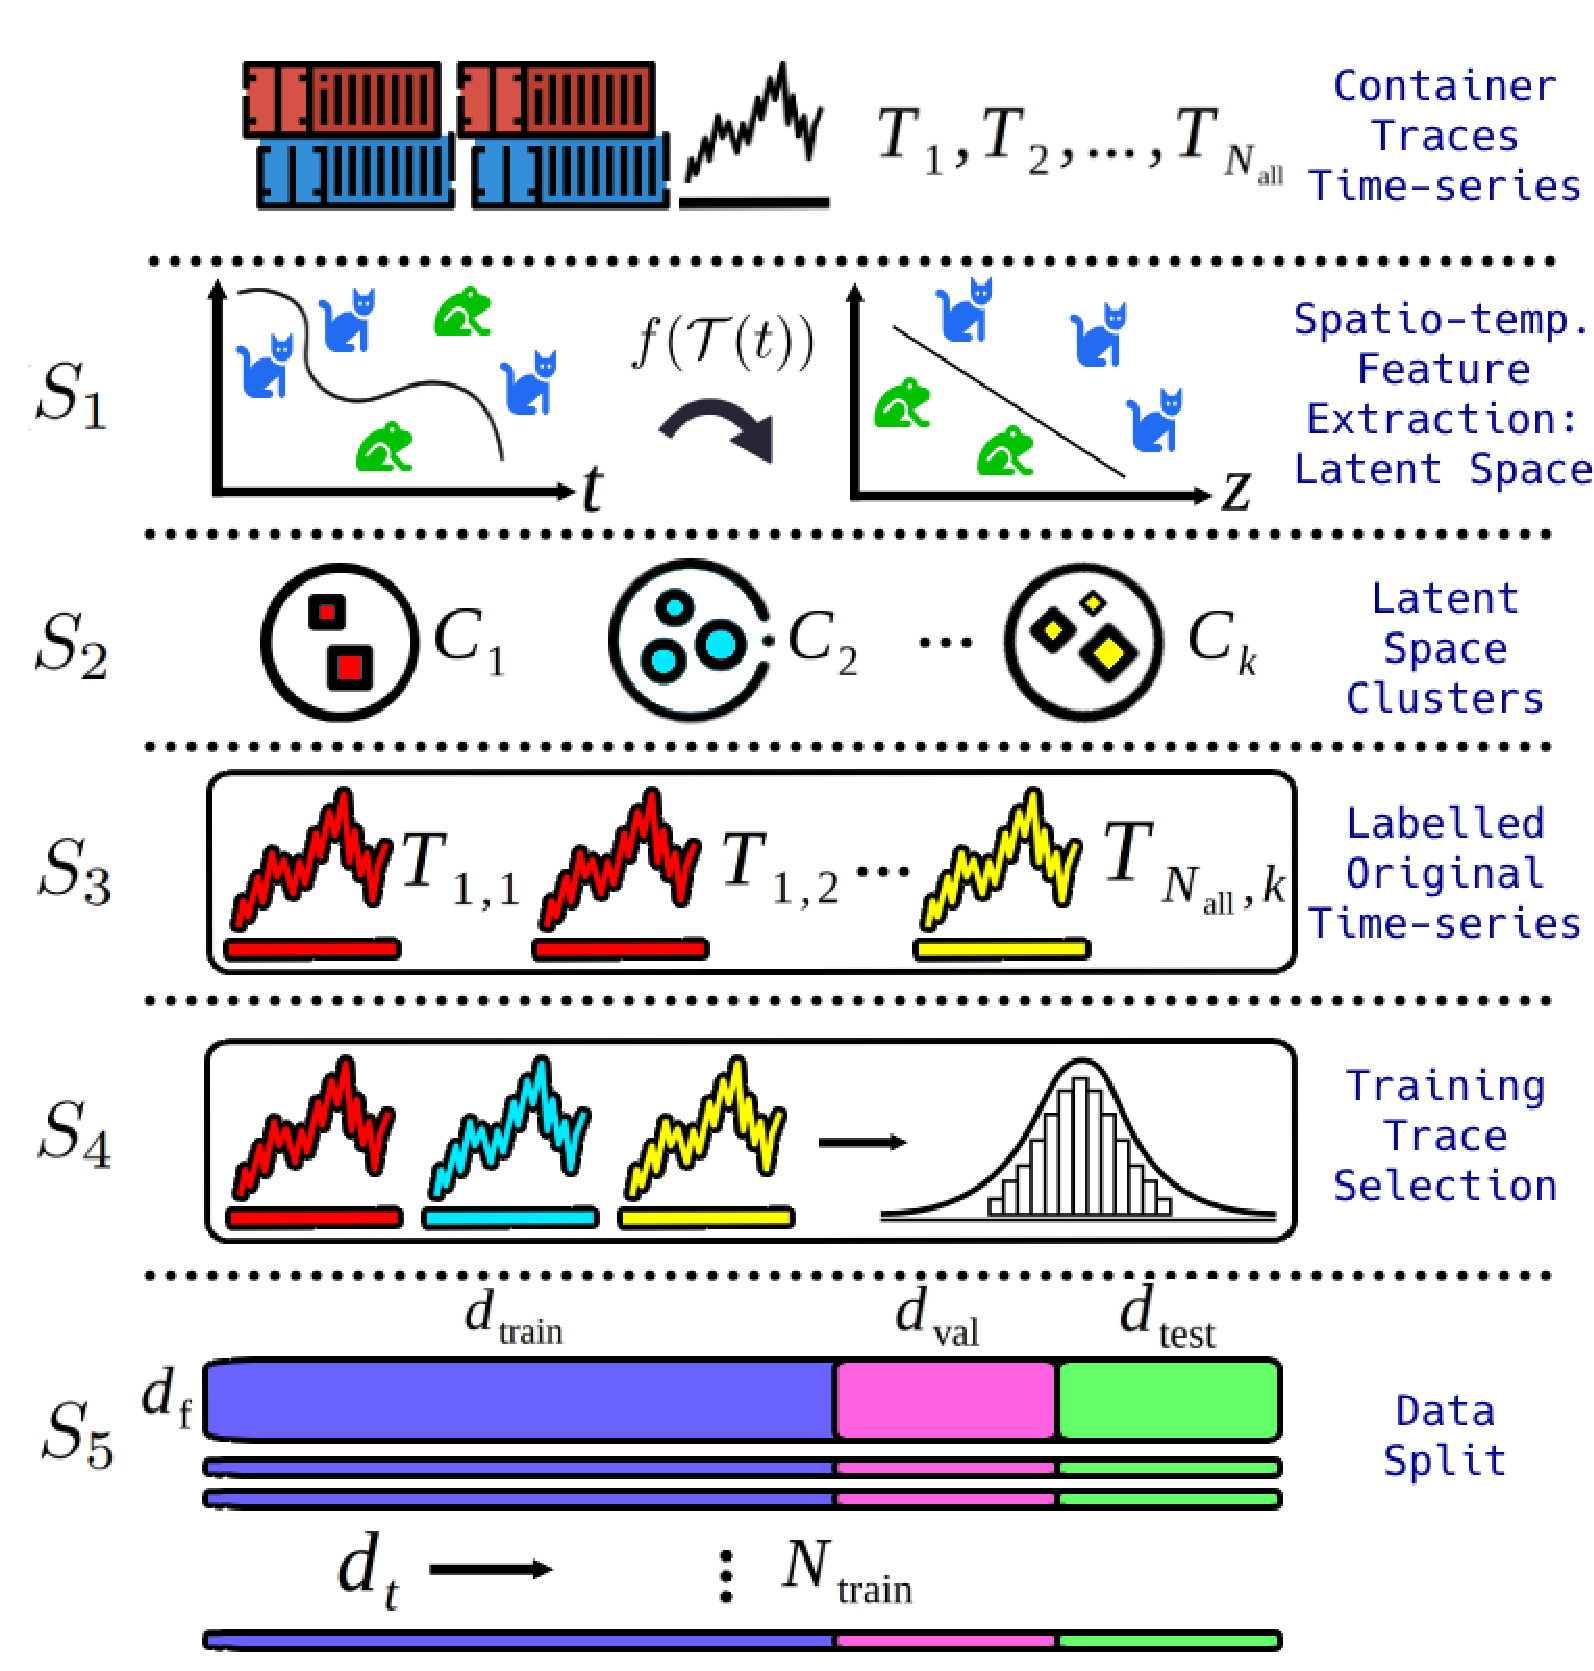
\includegraphics[width=0.49\textwidth]{img/proposed_solution_trace_selection.pdf}
\caption{Trace sampling process for generalization training. Historical workload data are processed to extract container traces, which are clustered into representative groups.}
\label{fig:proposed_solution_trace_selection}
\end{figure}

To achieve robust generalization across diverse workloads, OmniFORE employs a novel approach to extract a representative set of historical traces from the edge-cloud network. This strategy ensures that the model trained on these traces can effectively generalize to various workload types. The detailed steps ($S_1$ - $S_5$) of this process are outlined in Fig. ~\ref{fig:proposed_solution_trace_selection}.

The goal of these steps is to extract a \textbf{set of historical traces}, denoted as \(\mathbf{T}_{\text{train}}(t)\), where \(N_{\text{train}}\) represents the number of training traces. This set is a representative subset of the entire set of traces, \(\mathbf{T}_{\text{all}}(t)\), which contains \(N_{\text{all}}\) traces. "Representative" means that \(\mathbf{T}_{\text{train}}(t)\) captures the essential characteristics and variations present in \(\mathbf{T}_{\text{all}}(t)\), ensuring that the training set accurately reflects the diversity and distribution of the full dataset:

\begin{equation}
\mathbf{T}_{\text{train}}(t) \in \mathbb{R}^{d_f \times d_t \times N_{\text{train}}} \subset \mathbf{T}_{\text{all}}(t) \in \mathbb{R}^{d_f \times d_t \times N_{\text{all}}},
\end{equation}
where $N_{\text{train}} < N_{\text{all}}$. Using all traces for training would be computationally prohibitive and costly.

Section \ref{sec: Container Trace Heterogeneity} underscores the diverse workloads handled by containers, which require efficient resource management through OmniFORE. The highly dynamic nature of container data, marked by their time-dependent spatio-temporal patterns, presents significant challenges for analysis. Traditional clustering algorithms often struggle with such complex time-series data \cite{gupta2020approaches}. To overcome this, we propose transforming the data into a latent space to create a dense representation, facilitating more efficient clustering and differentiation \cite{frazier2018tutorial}. This latent space captures essential features, enabling better management of the data's complexities.

First ($S_1$), OmniFORE extracts spatio-temporal features from the container trace time-space, denoted as $\mathcal{T}$. Each trace $T_i(t) \in \mathbb{R}^{d_f \times d_{\text{t}}}$ is then transformed into \textbf{a lower-dimensional latent space}, $\mathcal{Z} \in \mathbb{R}^{z}$, where $z \ll d_f \times d_t$. This transformation, defined as $\mathcal{Z}(z) = f_{\text{encoder}}(\mathcal{T}(t))$, is optimized to capture the essential spatio-temporal patterns of the data over time. Details are provided in Section \ref{sec: Unsupervised Temporal Clustering}. By converting the time-dependent space $\mathcal{T}$ into the latent space $\mathcal{Z}$, OmniFORE optimizes for the most informative features for clustering, enhancing both efficiency and effectiveness by reducing dimensionality while preserving essential temporal information.

Second ($S_2$), the latent space $\mathcal{Z}$ is then \textbf{clustered}. Each cluster $C_k$ groups all container traces with similar spatio-temporal patterns over time into $K$ groups. The clustering process can be represented as
\begin{equation}   
\{C_1, C_2, \ldots, C_K\} = \text{Cluster}(\mathcal{Z}(z)).
\end{equation}
Third ($S_3$), each cluster \(C_k\) labels the original time-series traces, preserving the unique characteristics of each trace for accurate model training while leveraging the efficiency of latent space clustering. This can be mathematically depicted as
\begin{equation}
\mathbf{T}_{\text{all, cluster}}(t) = \{T_{1,1}(t), T_{2,1}(t), \ldots, T_{N_\text{all},k}(t)\},
\end{equation}
where $T_{1,1}(t)$ denotes the first trace in cluster 1.

Fourth ($S_4$), \textbf{representative traces} from each cluster $C_k$ are selected for training the prediction model. The selection process is optimized to ensure that the training data is diverse and representative of the broader dataset. Given a total number of traces $N_{\text{all}}$ and a desired subset of $N_{\text{train}}$ traces, the selection process is proportional to the number of traces in each cluster.

Let $N_{C_k}$ denote the number of traces in cluster $C_k$. The proportion of traces in each cluster compared to the total number of traces is
\begin{equation}
p_k = \frac{N_{C_k}}{N_{\text{all}}} \in \left[ 0, 1 \right].
\end{equation}
The number of traces selected from each cluster $C_k$ for the training set is
\begin{equation}
N_{\text{train},k} = \left\lfloor p_k \cdot N_{\text{train}} \right\rfloor,
\end{equation}
where $N_{\text{train},k}$ is the number of traces selected from cluster $C_k$ for training.

Therefore, the total number of traces in the training set $T_{\text{train}}$ is the sum of the selected traces from each cluster, such that

\begin{equation}  
N_{\text{train}} = \sum_{k=1}^{K} N_{\text{train},k}.
\end{equation}

%% data split
Finally ($S_5$), the traces in the sampled training set are split into train/validation/test segments along the time dimension ($d_t = d_{\text{train}} + d_{\text{val}} + d_{\text{test}}$), resulting in:

\begin{equation}
\begin{equation*}
aligned
\end{equation*} 
\end{equation}

OmniFORE ensures that data is effectively utilized for training, validating, and testing the prediction models, resulting in robust and generalizable performance.

\subsection{Unsupervised Temporal Clustering}
\label{sec: Unsupervised Temporal Clustering}

Figure \ref{fig:latent_space_creation} provides an overview of the \textbf{latent space extractor}. The input time-series $\mathcal{T}(t)$ is transformed into a latent space $\mathcal{Z}(z)$ by the encoder function $f_{\text{encoder}}$. The decoder function $f_{\text{decoder}}$ then reconstructs $\mathcal{Z}(z)$ into the output time-series $\mathcal{R}(t)$, which approximates $\mathcal{T}(t)$. This neural network structure compresses the data into a latent space, captures its critical features, and then reconstructs the original data. Successful reconstruction with the latent space acting as a \textbf{bottleneck} indicates that the latent space effectively encapsulates the essential information of the input signal.

To utilize this dense representation, we modify a \textbf{supervised} (using correct cluster labels for each trace) CNN-based approach for time-series clustering from \cite{clusteringDL} to an \textbf{unsupervised} (without cluster labels) version within OmniFORE. This process involves feature extraction through convolutional and pooling operations on raw data, followed by clustering in the latent space.

% Fig. \ref{fig:2d_latent_space} shows a 2D Principal Component Analysis \cite{abdi2010principal} of clusters in the latent space, where each point represents a time-series trace, color-coded by cluster.

\begin{figure}\centering
\centering
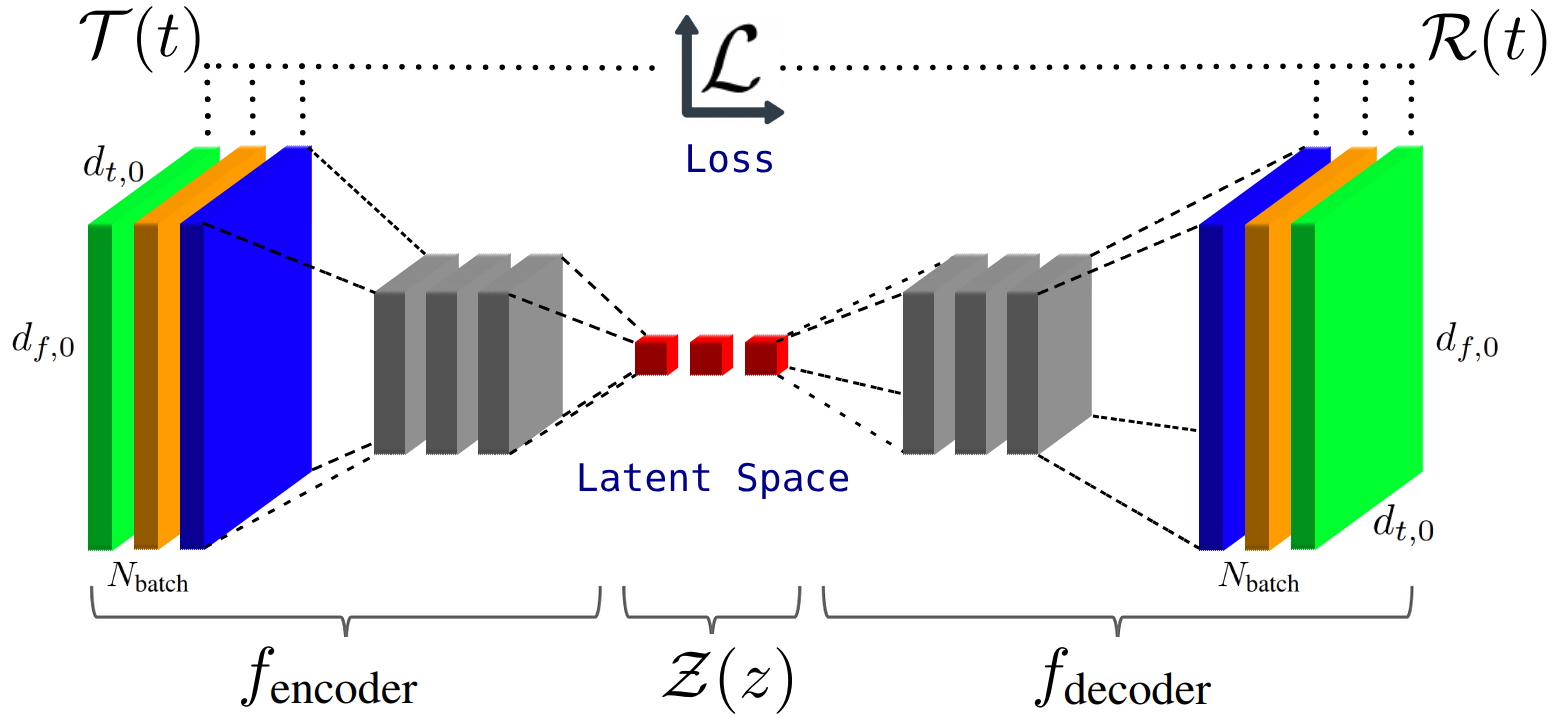
\includegraphics[width=0.49\textwidth]{img/latent_space_creation.png}
\caption{Overview of the latent space extractor. The input $\mathcal{T}(t)$ is encoded into latent space $\mathcal{Z}(z)$ by $f_{\text{encoder}}$ and then decoded by $f_{\text{decoder}}$ to reconstruct $\mathcal{R}(t) \approx \mathcal{T}(t)$.}
\label{fig:latent_space_creation}
\end{figure}

The architecture of the latent space extractor comprises the following layers:
\begin{enumerate}
    \item \textbf{Encoder}: Transforms an input trace $T_i$ into the latent space $\mathcal{Z}(z)$ using $\mathcal{Z}(z) = f_{\text{encoder}}(\mathcal{T}(t))$.
    \begin{itemize}
        \item \textbf{Input Layer}: \(d_{f,0} \times d_{t,0}\) neurons, where \(d_{t,0}\) is the series length and \(d_{f,0}\) is the number of features.
        \item Several repetitions \(r\) of combined convolutional and pooling layers, where \(d_{f,r}\) is the number of filters and \(d_{t,r}\) is the size of the sequence dimension after the \(r\)-th convolutional layer. The transformed sequence is \(T'(t') \in \mathbb{R}^{d_{f,r} \times d_{t,r} \times N_{\text{all}}}\).
        \begin{itemize}
            \item \textbf{Convolutional Layers ${\boldsymbol{C}}_{r}(t')$}: Parameters are convolution stride ($s_r$), filter size ($d_{f,r-1} \times l_r$), activation functions, trainable weights ($\boldsymbol{\omega}_r$), and biases ($\boldsymbol{b}_r$).
            \item \textbf{Pooling Layers $\boldsymbol{P}_r(t')$}: Downsampling strategy to reduce feature map size by averaging regions.
        \end{itemize}
        \item \textbf{Latent Space Layer}: Converts the flattened output of the last convolutional layers, $\boldsymbol{C}_r$, into a lower-dimensional latent space, $\mathcal{Z} \in \mathbb{R}^{z \times N_{\text{batch}}}$, where $z \ll d_{f,0} \times d_{t, 0}$.
    \end{itemize}
    \item \textbf{Decoder}: Converts $\mathcal{Z}(z)$ back to $\mathcal{T}(t)$ as $\mathcal{R}(t) = f_{\text{decoder}}(\mathcal{Z}(z)) \approx f_{\text{encoder}}^{-1}(\mathcal{Z}(z))$.
        \begin{itemize}
            \item \textbf{Multiple Transposed Convolution Layers}: Reconstruct the time-series input data from the latent representation, back to the original data shape. Transposed convolutions, also known as deconvolutions, upsample the input by reversing the operations of standard convolutional layers.
        \end{itemize}
\end{enumerate}
The training process can be described as:
\begin{enumerate}
    \item \textbf{Initialize}: Set up the Encoder-Decoder architecture, initialize weights and biases.
    \item \textbf{Load Input Data}: Prepare input traces as $\mathbf{T_{\text{all}}} \in \mathbb{R}^{ d_{t,0} \times d_{f,0} \times N_{\text{all}}}$, split into $N_{\text{batch}}$ batches. Here, $N_{\text{batch}}$ denotes the number of batches.
    \item \textbf{Forward Pass}: Compute the output of each layer for each batch.
    
    \begin{itemize}
        \item \textbf{Encoder Convolution Layer}:
        \begin{footnotesize}
        \begin{equation}
        \boldsymbol{C}_r(t') = \sum_{i=1}^{l_r} \sum_{j=1}^{d_{f, r-1}} T^{'}_R(i+s_r(t'-1), j) \boldsymbol{\omega}_r(i, j) + \boldsymbol{b}(r),
        \end{equation}
        \end{footnotesize}
        where $\boldsymbol{\omega}_r \in \mathbb{R}^{l_r \times d_f}$ and $\boldsymbol{b}(r)$ are the weights and bias of the $r$-th convolution filter.
        
        \item \textbf{Encoder Pooling Layer}:
        \begin{footnotesize}
        \begin{equation}
        \boldsymbol{P}_r(t') = \operatorname{MaxPool}\left(\boldsymbol{C}_r((t'-1)l_r+1), \ldots, \boldsymbol{C}_r(t' l_r)\right).
        \end{equation}
        \end{footnotesize}
        \item \textbf{Decoder}: Transposed convolutions for reconstruction.
    \end{itemize}
    \item \textbf{Loss Function}: Calculate the mean-square error across all batches between the reconstructed time-series and the actual input time-series as
    \begin{equation}
    \mathcal{L} = \frac{1}{2N_{\text{batch}}} \sum_{n=1}^{N_{\text{batch}}} \sum_{t=1}^{d_t} \Big(T_i(t) - R_i(t) \Big)^2.
    \end{equation}
    \item \textbf{Update}: Use gradient descent to update the weights and biases of the (transposed) convolutions ($\boldsymbol{\omega}_r$, $\boldsymbol{b}_r$) and optimize for minimizing the loss function.
    \item \textbf{Iterate}: Repeat with new batches until the model converges.
\end{enumerate}

This unsupervised approach compresses time-series data into a latent space, capturing essential features and enabling reconstruction. By adapting CNN-based clustering to work without labels, it achieves efficient feature extraction for selecting appropriate model training traces.

\subsection{Attention Mechanism for Extended Sequences}

The original transformer model \cite{vaswani2017attention} significantly enhances dependency capture, yet faces computational hurdles with long sequences \cite{wen2022transformers}. Recent developments in efficient transformers \cite{fasterandlightertransformers} and sparse attention techniques \cite{gorbett2023sparse, STRec, ma2024multivariate} mitigate these issues. Within OmniFORE, we utilize informers \cite{zhou2021informer}, which leverage sparse attention mechanisms to predict extensive time-series data efficiently. Informers are a viable alternative to traditional transformers, despite their implementation complexity, and a crucial element of our proposed solution.

\begin{figure}\centering
\centering
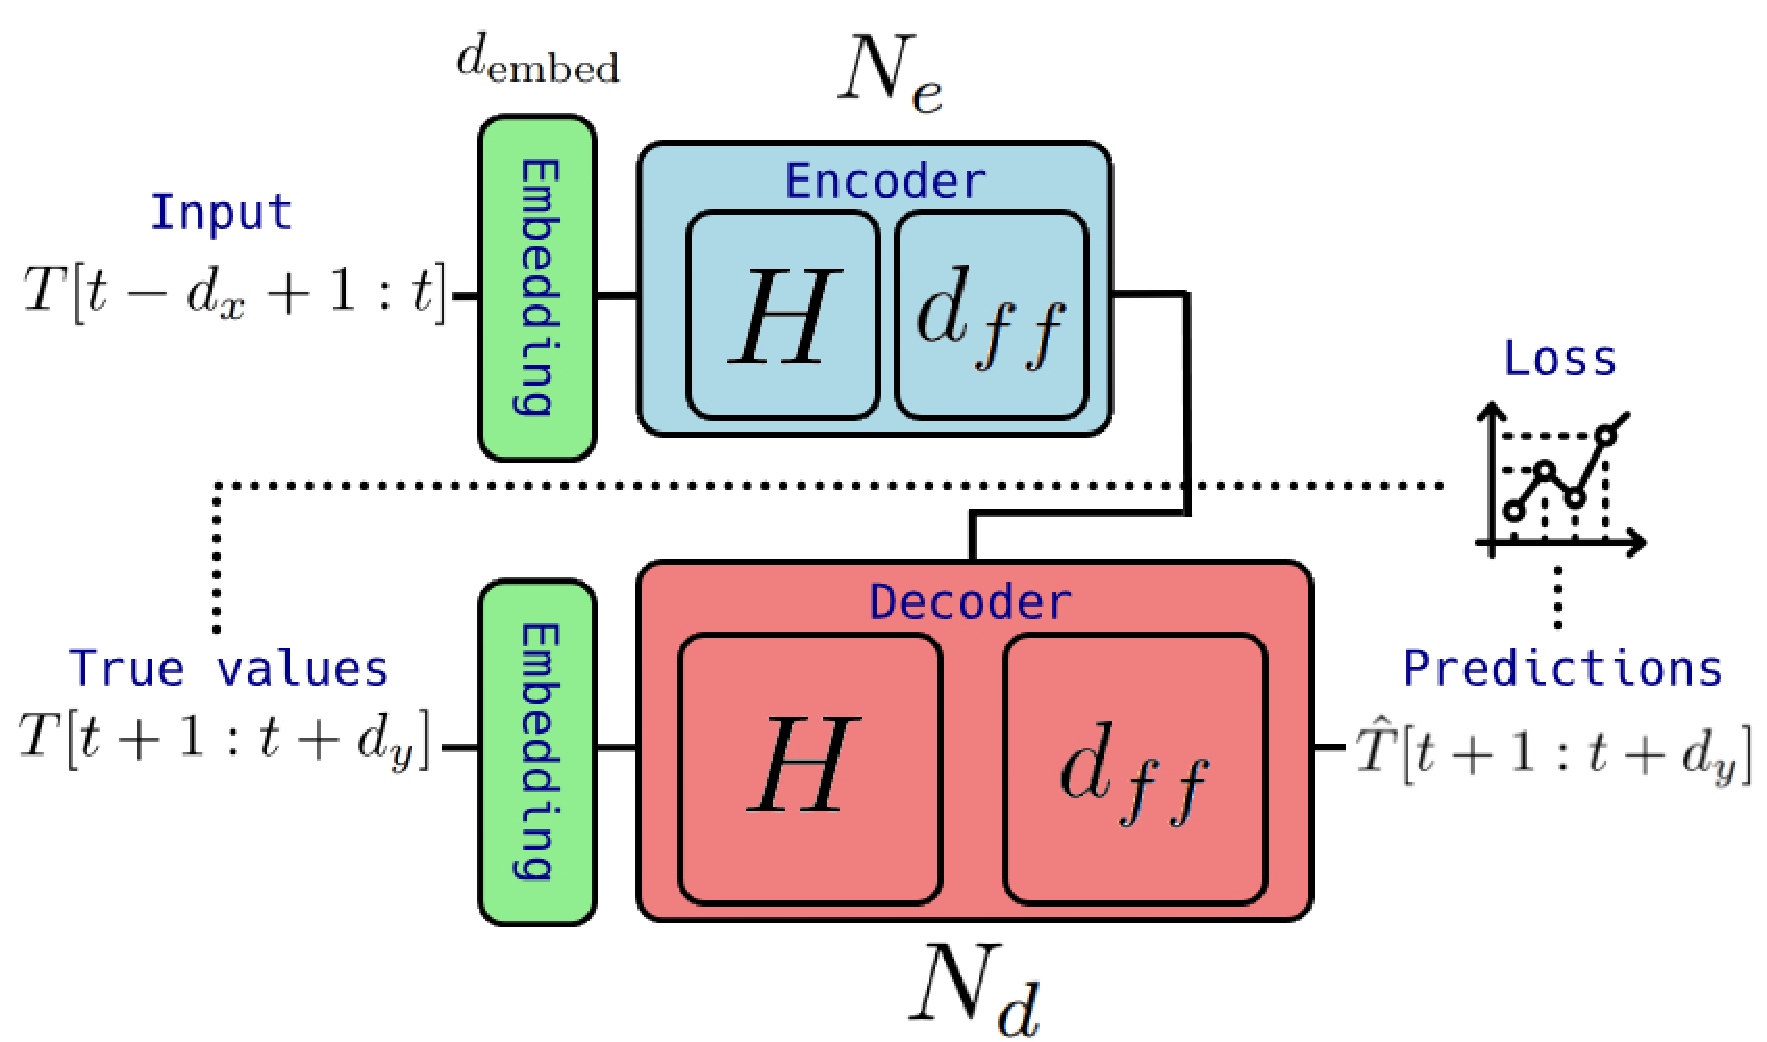
\includegraphics[width=0.49\textwidth]{img/Transformer_Architecture.pdf}
\caption{High-level overview of the transformer architecture}
\label{fig:Transformer_Architecture}
\end{figure}

Figure \ref{fig:Transformer_Architecture} outlines the vanilla transformer architecture, comprising an encoder and decoder. The input sequence $T[t-d_x:t]$ is embedded into a higher-dimensional space $d_{\text{embed}}$. The encoder, with $N_e$ layers (repetitions of the complete block), applies self-attention ($H$) and feed-forward networks ($d_{ff}$) to capture dependencies. The decoder, with $N_d$ layers, generates predictions $\hat{T}[t+1:t+d_y]$ by attending to both encoded inputs and previous outputs. In the following sections, we provide a high-level understanding of this architecture, which covers both transformers and the informers.

\subsubsection*{Time-series Embedding}

The \texttt{DataEmbedding}, denoted as $\mathbf{E}$, combines three embeddings to form a robust representation of time-series input sequence. The \texttt{Value Embedding} \cite{yue2022ts2vec} maps raw input values to a higher-dimensional space via a convolutional layer, capturing intricate data patterns of the input sequence. The \texttt{Positional Embedding} \cite{kazemnejad2024impact} encodes the sequence order using sinusoidal functions, preserving structural information crucial for time-series analysis. The \texttt{Temporal Embedding} \cite{liu2023spatio} incorporates time-related features (e.g., hour, day) to provide context on temporal dependencies and seasonal trends. These components are summed to produce the final embedding matrix $\mathbf{E}$, as described in the equation:

\begin{equation}
\mathbf{E} = \mathbf{E}_{\text{value}} + \mathbf{E}_{\text{position}} + \mathbf{E}_{\text{temporal}} \in \mathbb{R}^{d_x \times d_{\text{embed}}}.
\end{equation}

This matrix serves as the input to the subsequent layers of the model, encapsulating both the intrinsic data patterns and the temporal structure of the time-series.

\subsubsection*{Introduction to Attention Mechanism}

\begin{figure}\centering
\centering
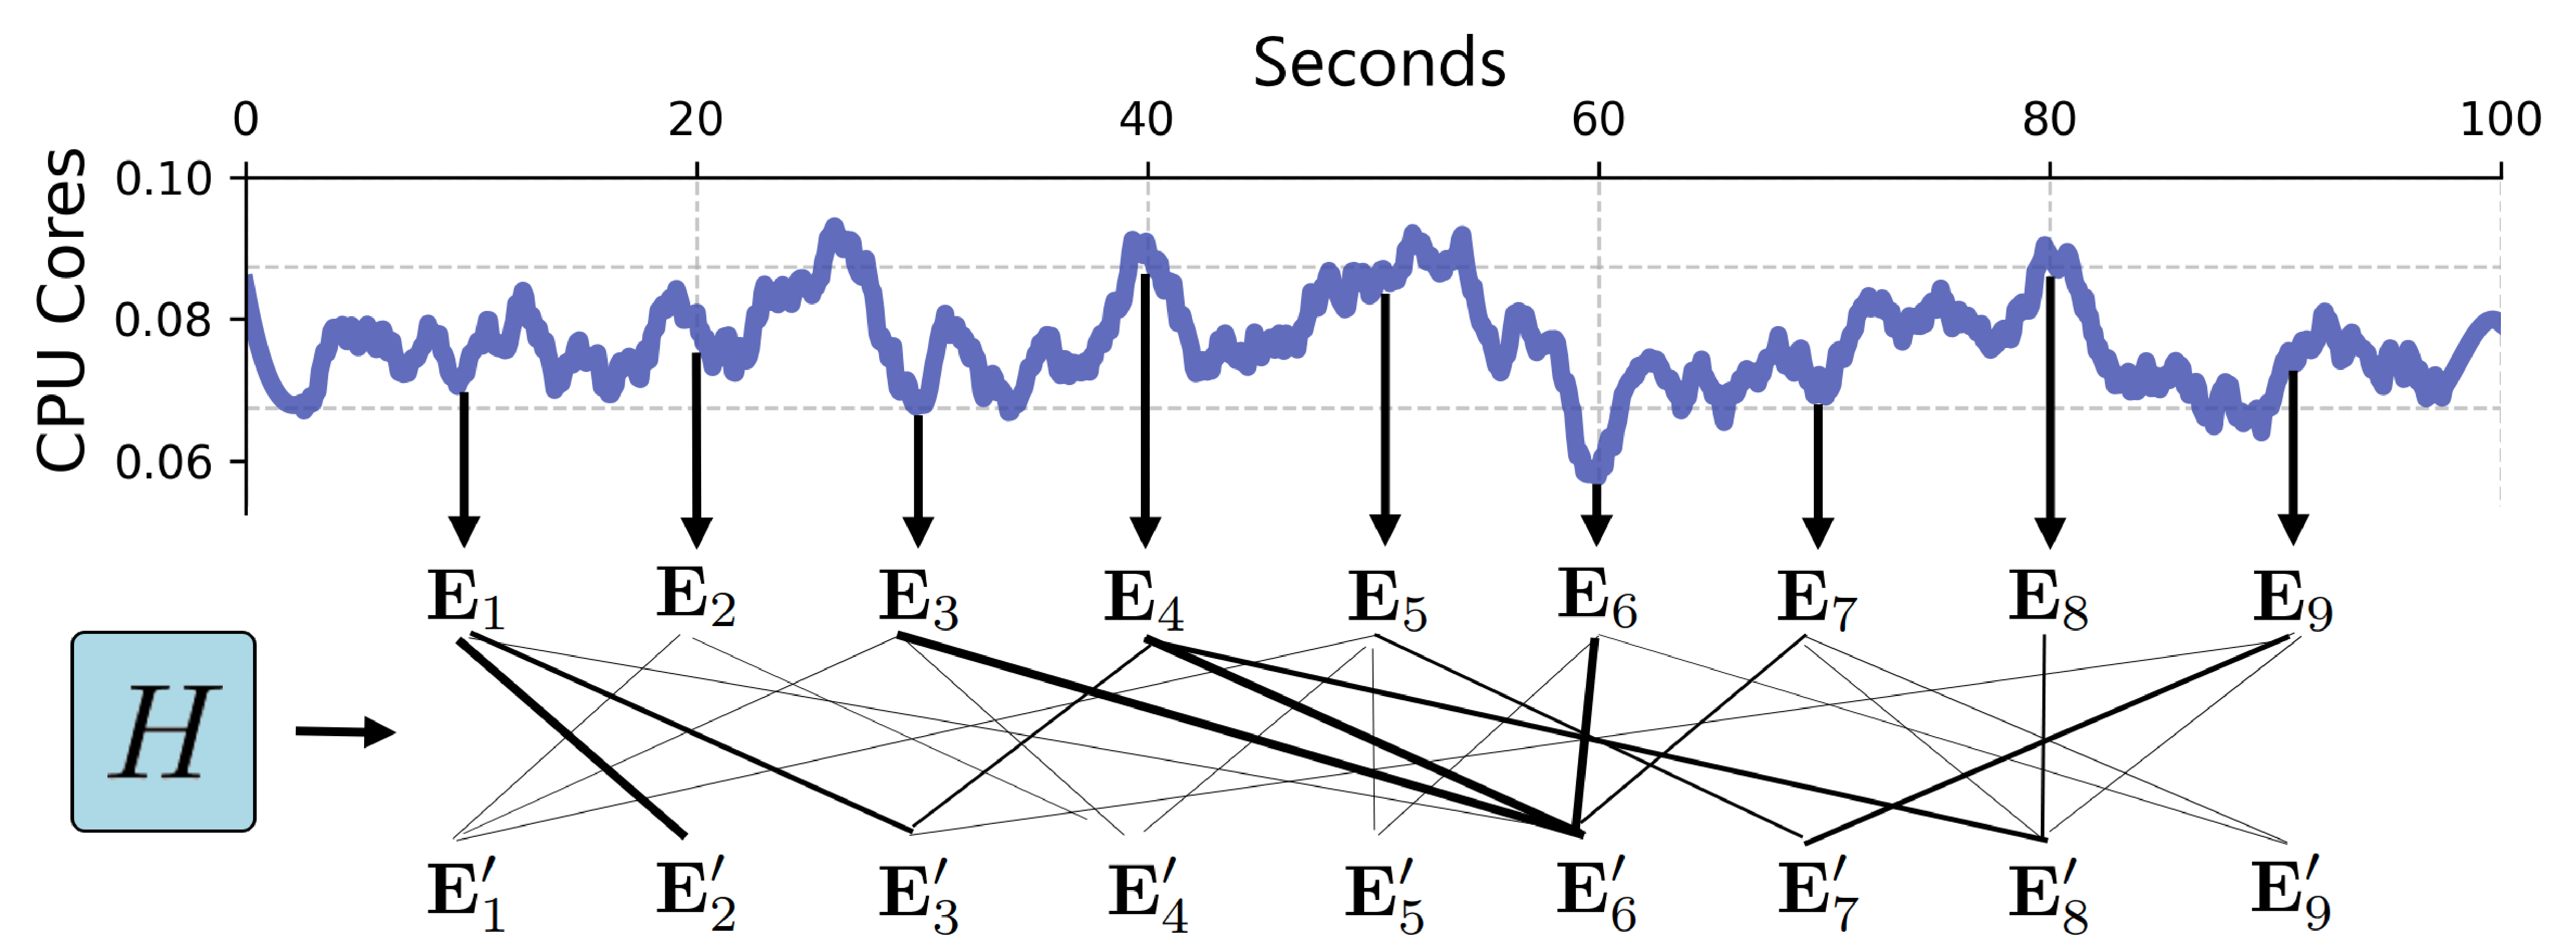
\includegraphics[width=0.49\textwidth]{img/attention_goal.pdf}
\caption{Attention mechanism refining time-series embeddings $\mathbf{E}_i$ to $\mathbf{E}_i'$, with arrow thickness indicating the strength of influence.}
\label{fig:attention_goal}
\end{figure}

Starting with the initial embeddings $\mathbf{E} \in \mathbb{R}^{d_x \times d_{\text{embed}}}$, the attention mechanism (denoted as $\mathcal{A}$) refines these embeddings into a new set, $\mathbf{E}'$ \cite{vaswani2017attention}. This mechanism enables the model to selectively focus on specific time steps, analogous to human attention. For instance, when predicting future workload at a peak, both the model and a human analyst would focus on the pattern surrounding the current peak and compare it to similar peaks in the past. The attention weights determine the degree to which each original embedding $\mathbf{E}i \in \mathbb{R}^{d{\text{embed}}}$ contributes to its corresponding refined embedding $\mathbf{E}_i'$. As illustrated in Fig. \ref{fig:attention_goal}, thicker lines indicate stronger influence. The refined embeddings $\mathbf{E}'$ effectively combine underlying data patterns with temporal relationships, enhancing the model's capacity to capture complex dependencies across the sequence \cite{dai2019transformer}.

To construct the refined embeddings $\mathbf{E}_i'$, the attention mechanism employs three key components: queries, keys, and values \cite{vaswani2017attention}, as illustrated in Fig. \ref{fig:attention_workings}. The model transforms each embedding $\mathbf{E}_i$ into three vectors:

\begin{equation}
    \begin{equation*}
aligned
\end{equation*}
\end{equation}
where $\mathbf{W_Q}, \mathbf{W_K}, \mathbf{W_V} \in \mathbb{R}^{d_{\text{embed}} \times d_{\text{embed}}}$ are learned weight matrices. Conceptually, a query vector encodes the information need at the current time step, key vectors facilitate the identification of relevant past information, and value vectors contain the actual content to be aggregated \cite{bahdanau2014neural}. In the context of workload prediction, when analyzing a peak, the query vector would encode features of the current peak, key vectors would help identify similar historical peaks, and value vectors would contain the associated historical workload patterns.

The model evaluates temporal relationships by computing scaled dot products between query and key vectors:

\begin{equation}
    \text{Score}(\mathbf{Q}_i, \mathbf{K}_j) = \frac{\mathbf{Q}_i \mathbf{K}_j^T}{\sqrt{d_{\text{embed}}}}.
\end{equation}

A high score indicates that the corresponding time step contains critical information for the current prediction, as the vectors align in high-dimensional space \cite{luong2015effective}. The scaling factor $\sqrt{d_{\text{embed}}}$ ensures training stability by preventing excessively large values that could lead to sharp, unbalanced distributions post-softmax \cite{xu2015show}. The softmax function normalizes these scores into a probability distribution, effectively assigning weights to each timestep's embedding vector. These weights, summing to one, determine the relative importance of each timestep, guiding the attention mechanism to focus on the most relevant parts of the sequence.

To capture diverse temporal dependencies, the model employs \textit{multi-headed attention} \cite{michel2019sixteen} with $H$ parallel attention mechanisms, or "heads" (Fig. \ref{fig:attention_workings}). Each head $h \in \{1, ..., H\}$ operates independently on the same input embeddings, but with its own set of learnable weight matrices $\mathbf{W}_Q^h, \mathbf{W}_K^h, \mathbf{W}_V^h \in \mathbb{R}^{d_{\text{embed}} \times d_{\text{head}}}$, where $d_{\text{head}} = d_{\text{embed}} / H$. These matrices are initialized differently, leading to distinct evolutionary trajectories during training and convergence to different local optima~\cite{zhang2019improving}. This architectural design enables the model to simultaneously project the input into multiple subspaces and attend to various aspects of the sequence, such as short-term fluctuations and long-term trends, effectively increasing the model's representational capacity without a proportional increase in computational complexity \cite{vaswani2017attention}.

For each head $h$, the attention output is computed as

\begin{equation}
    \mathbf{A}_i^h = \mathcal{A}(\mathbf{E}_i\mathbf{W}_Q^h, \mathbf{E}_i\mathbf{W}_K^h, \mathbf{E}_i\mathbf{W}_V^h).
\end{equation}

The outputs from all heads are concatenated and linearly transformed to produce the multi-headed attention output

\begin{equation}
    \mathbf{MHA}_i = d_{ff}(\operatorname{Concat}(\mathbf{A}_i^{(1)}, \mathbf{A}_i^{(2)}, \ldots, \mathbf{A}_i^{(H)})),
\end{equation}
where $d_{ff}: \mathbb{R}^{d_{\text{embed}} \times H} \rightarrow \mathbb{R}^{d_{\text{embed}}}$ represents a linear transformation layer. This layer projects the concatenated attention outputs from all $H$ heads, with total dimension $d_{\text{embed}} \times H$, back to the original embedding dimension $d_{\text{embed}}$.

The final refined embedding for each time step incorporates a residual connection \cite{he2016deep} and layer normalization \cite{lei2016layer}:

\begin{equation}
    \mathbf{E}_i' = \text{LayerNorm}(\mathbf{E}_i + \mathbf{MHA}_i),
\end{equation}
where LayerNorm denotes layer normalization. This is followed by a position-wise feed-forward network ($d_{ff}$) with another residual connection and layer normalization:

\begin{equation}
    \mathbf{E}_i'' = \text{LayerNorm}(\mathbf{E}_i' + d_{ff}(\mathbf{E}_i')).
\end{equation}

This entire process—multi-headed attention, residual connections, layer normalizations, and feed-forward network—constitutes one layer of the transformer encoder. It is repeated across multiple stacked layers ($N_e$). Each layer operates on the output of the previous one, allowing for iterative refinement of embeddings and progressively developing intricate representations crucial for accurate predictions in complex time-series tasks.

\begin{figure}\centering
\centering
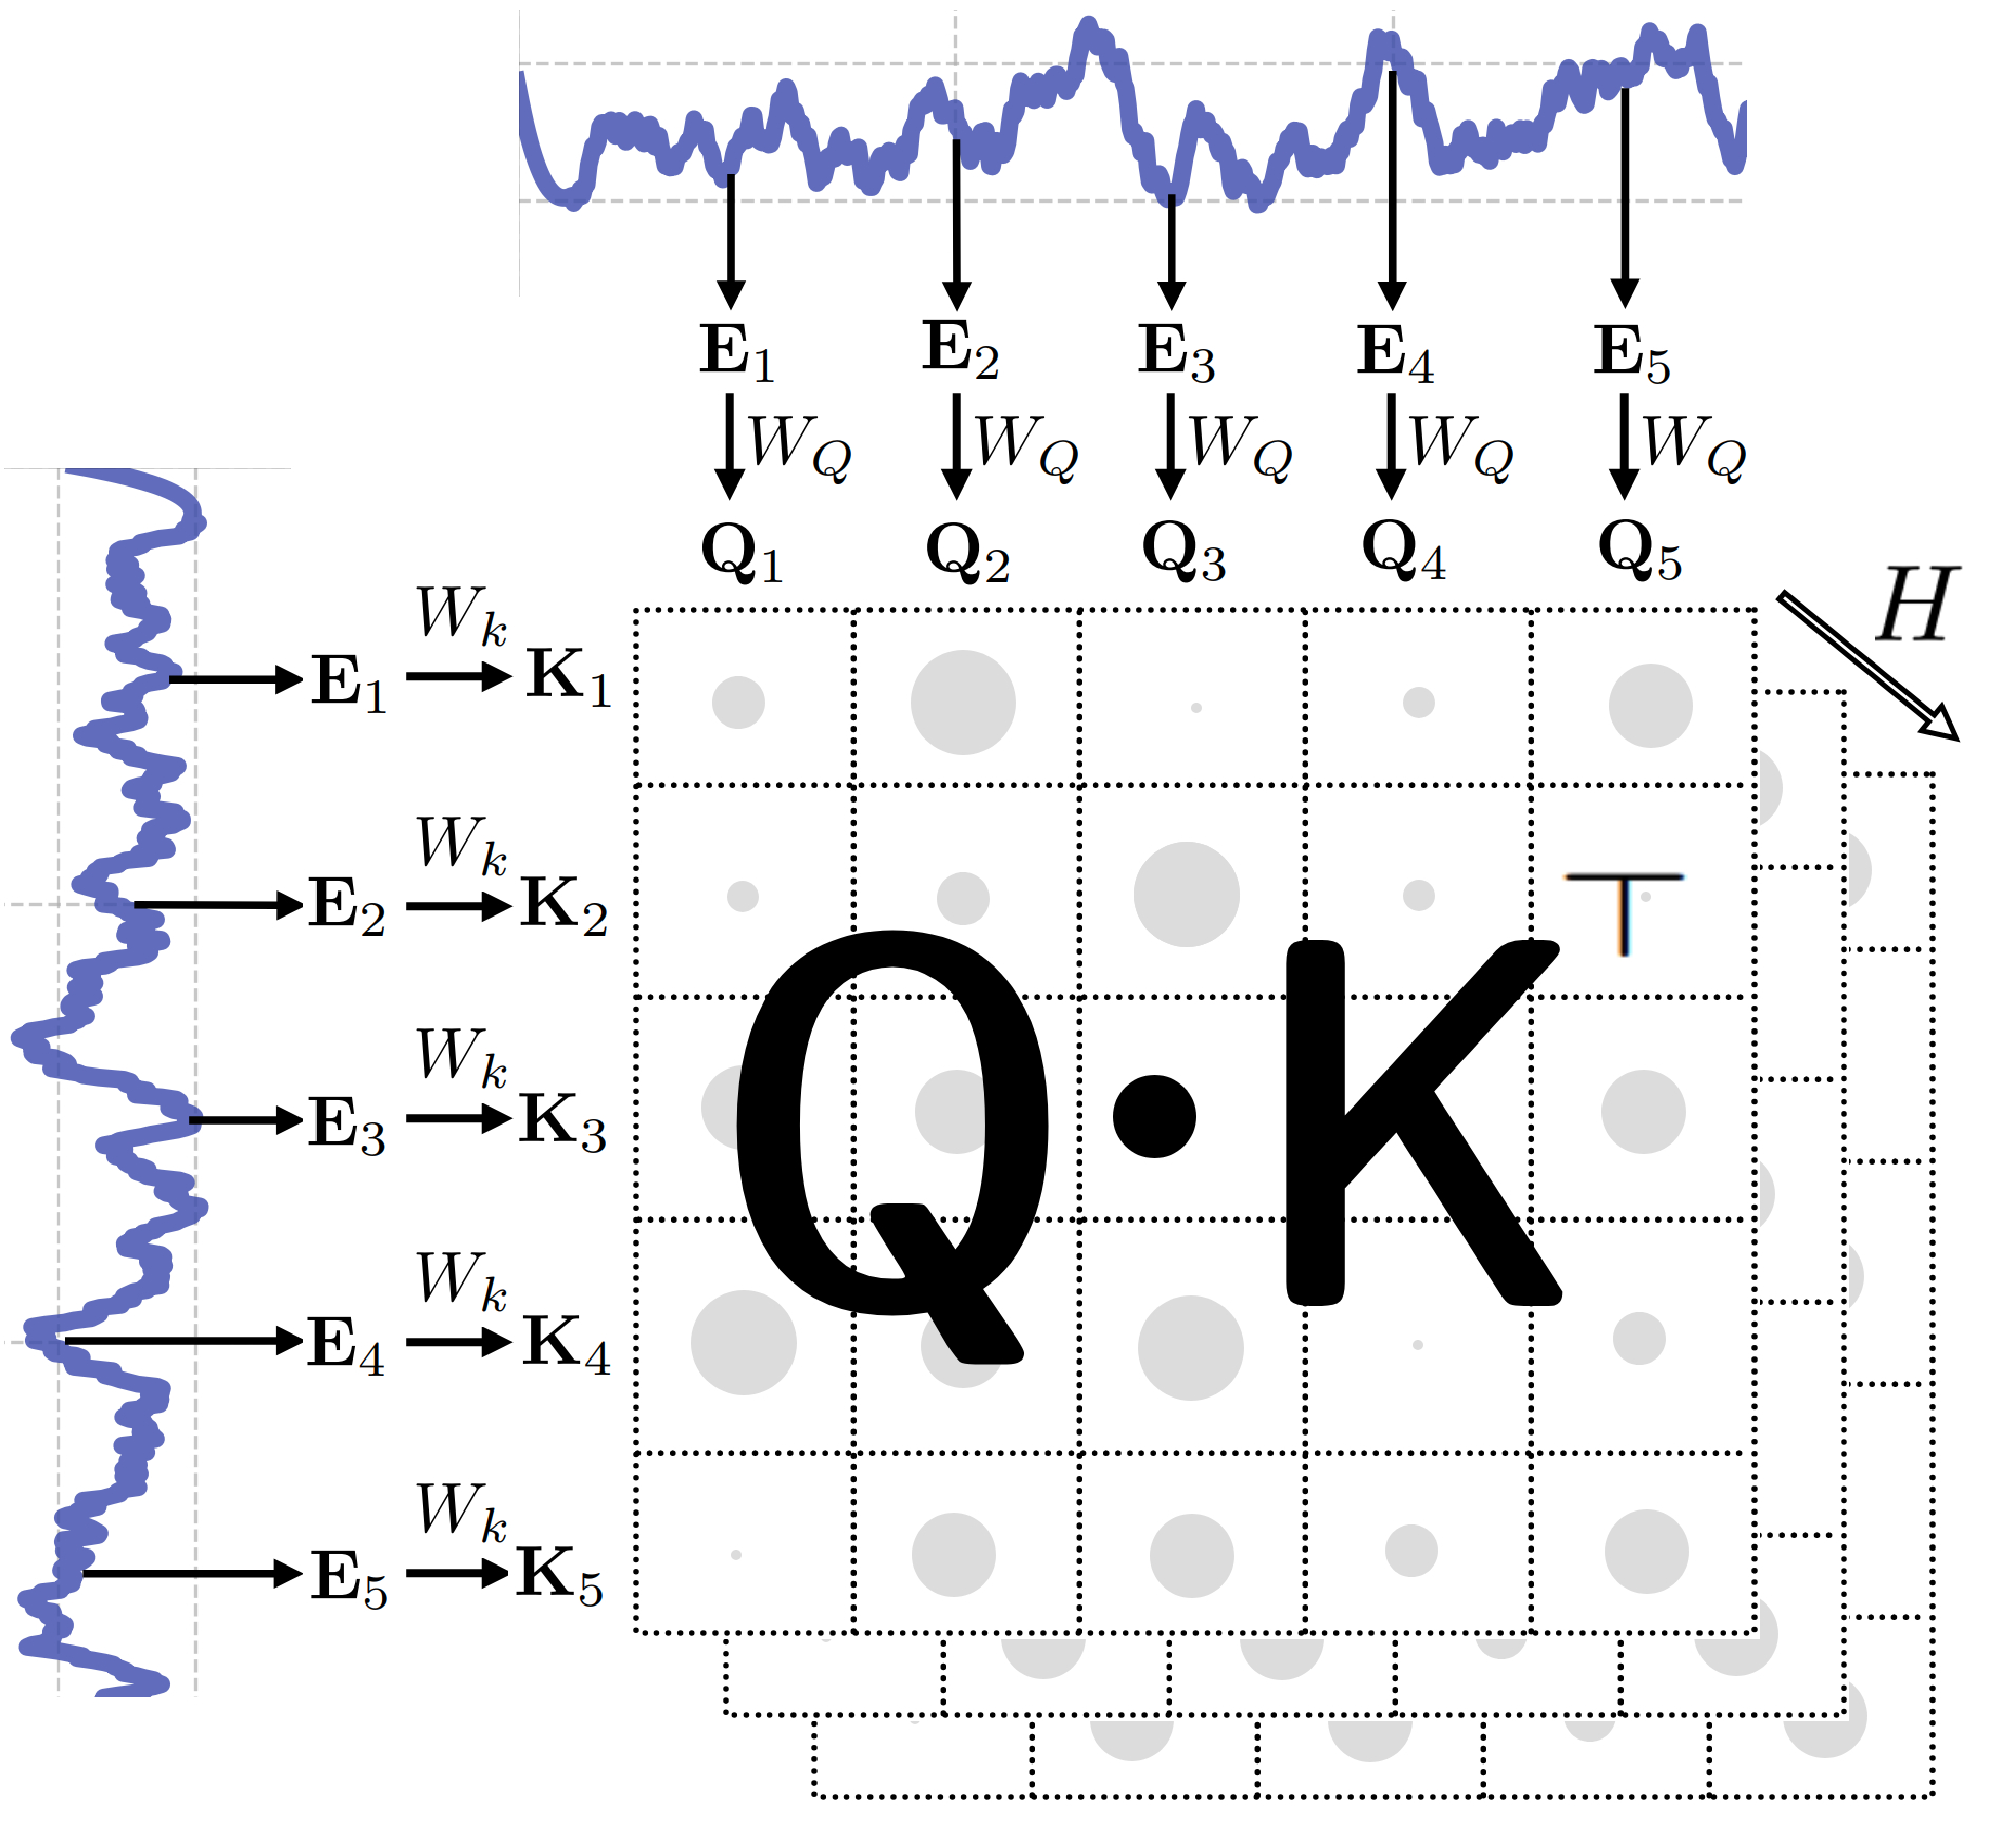
\includegraphics[width=0.42\textwidth]{img/attention_workings.pdf}
\caption{Multi-Headed Attention: Input embeddings ($\mathbf{E}_i$) are transformed into query ($\mathbf{Q}$), key ($\mathbf{K}$), and value ($\mathbf{V}$) vectors. Multiple heads ($H$) capture different temporal aspects. Larger circles indicate stronger attention scores.}
\label{fig:attention_workings}
\end{figure}

\subsubsection*{Traditional Attention Mechanism}

The original self-attention mechanism \cite{vaswani2017attention} is defined by

\begin{equation}
\mathcal{A}(\mathbf{Q}, \mathbf{K}, \mathbf{V}) = \operatorname{Softmax}\left(\frac{\mathbf{QK}^\top}{\sqrt{d_{\text{embed}}}}\right) \mathbf{V},
\end{equation}
where $\mathbf{Q}, \mathbf{K}, \mathbf{V} \in \mathbb{R}^{d_x \times d_{\text{embed}}}$ are the query, key, and value matrices, respectively, while $d_{\text{embed}}$ is the embedding dimension of each point in the input sequence of length $d_x$. The product $\mathbf{QK}^\top \in \mathbb{R}^{d_x \times d_x}$ measures the importance of relationships between every data point in the sequence. This attention mechanism has $\mathcal{O}(d_x^2)$ complexity, making it inefficient for long input sequences.


\subsubsection*{Efficient Attention Mechanism}

The three architectural innovations of informers compared to the original transformer can be summarized as follows:
\subsubsection*{$\text{Informer}^{+1}$: Computationally Efficient Attention}

The sparse self-attention mechanism enhances efficiency by concentrating on the most critical queries. This is done by forming a sparse matrix $\overline{\mathbf{Q}}$ that retains only the most influential queries from $\mathbf{Q}$, with other entries set to zero. The selection of these important queries is directed by a sparsity measurement \cite{zhou2021informer}. This method significantly reduces computational complexity, making it more suitable for long sequences, as it scales linearly with the natural logarithm of the sequence length: $\mathcal{O}(d_x \log d_x)$.

\subsubsection*{$\text{Informer}^{+2}$: Memory Saving with Attention Distilling}

Due to the presence of zeros in the input matrix $\overline{\mathbf{Q}}$, the attention matrix $\mathcal{A}$ contains unnecessary entries. Removing these zero entries conserves memory and enables the model to concentrate on significant entries, a process known as attention distilling.

In each attention layer, the encoder utilizes self-attention distilling to minimize memory consumption by emphasizing the dominant entries in the attention matrix, thereby generating a new matrix

\begin{equation}
\mathcal{A}_{\text{distil}} = \operatorname{MaxPool}\left(\operatorname{ELU}\left(\operatorname{Conv1d}\left(\mathcal{A}\right)\right)\right),
\end{equation}
where $\operatorname{Conv1d}$ applies 1-D convolutional filters along the time dimension, and the activation function $\operatorname{ELU}$~\cite{al2023fhic} is used. The result is then passed through a max-pooling layer to downsample $\mathcal{A}$. This process decreases the time dimension of the input, reducing memory usage to $\mathcal{O}(d_x \log d_x)$.

\subsubsection*{$\text{Informer}^{+3}$: Fast Inference}

The decoder accelerates predictions for long sequences by utilizing generative inference, which forecasts the entire sequence in one step instead of predicting each time step sequentially. This is accomplished by using a known "start token" in conjunction with placeholders for the future sequence, formulated as

\begin{equation}
T_{\mathrm{de}}^{t} = \operatorname{Concat}\left(T_{\text{token}}^{t}, T_{\mathbf{0}}^{t}\right) \in \mathbb{R}^{(d_{\text{token}} + d_y) \times d_{\text{embed}}},
\end{equation}
where $T_{\text{token}}^{t} \in \mathbb{R}^{d_{\text{token}} \times d_{\text{embed}}}$ is the start token, and $T_{\mathbf{0}}^{t} \in \mathbb{R}^{d_y \times d_{\text{embed}}}$ acts as a placeholder for the future sequence. This generative inference approach significantly reduces computation time while preserving accuracy.



\subsection{Scaling}

Container traces in edge-cloud computing exhibit significant variability in resource usage, necessitating individual normalization to ensure balanced training. OmniFORE normalizes each trace such that the mean of the metric under study is zero (i.e., $\mu_i=0$) and the variance is one (i.e., $\sigma_i^2=1$), thereby preventing traces with higher means and variances from overshadowing others and enhancing model generalization.

Given a training set $\mathbf{T_{\text{train}}} \in \mathbb{R}^{d_t \times d_{\text{f}} \times N_{\text{train}}}$, each trace $T_i(t)$ is normalized as follows:

\begin{equation}
\tilde{T}_i(t) = \frac{T_i(t) - \mu_i}{\sigma_i},  
\end{equation}
where $\tilde{T}_i(t)$ denotes the normalized version of the trace $T_i(t)$, \(\mu_i\) is the mean, and \(\sigma_i = \sqrt{\sigma_i^2}\) is the standard deviation of the \(i\)-th trace. The mean \(\mu_i\) and variance \(\sigma_i^2\) are calculated as

\begin{equation}
\mu_i = \frac{1}{d_t} \sum_{t=1}^{d_t} T_i(t),   \sigma_i^2 = \frac{1}{d_t} \sum_{t=1}^{d_t} (T_i(t) - \mu_i)^2.
\end{equation}

The scaling parameters $(\mu_i, \sigma_i^2)$ are saved for each trace. During testing, these parameters are used to invert the normalization of predictions back to the original scale, such that

\begin{equation}
\hat{T}_i(t) = \tilde{T}_i(t) \cdot \sigma_i + \mu_i,
\end{equation}
where $i$ indexes each trace to maintain the scaling parameters for each trace.

\subsection{Bayesian Optimization with Generalization Objective}
\label{sec:BayesianOptimizationWithGeneralizationObjective}

Optimizing hyperparameters is essential for improving model performance and generalization \cite{hyperparamsdatasets}. Due to the impracticality of traditional grid search in expansive hyperparameter spaces \cite{gridsearchvsbayesian}, Bayesian optimization \cite{frazier2018tutorial} offers an efficient alternative by constructing a probabilistic model of the objective function and iteratively selecting the most promising hyperparameters.

Figure \ref{fig:gp_toy_example} illustrates Bayesian optimization, starting with initial observations (red dots) of the objective function. This simplified example reduces the hyperparameter space to prediction length $d_y$, though in practice it is multidimensional (hyperparameter vector $\mathbf{h}$). A model (blue line) predicts the objective function's mean and confidence interval (CI, shaded area). The next hyperparameter (star) is selected based on predicted high performance and uncertainty, balancing exploration and exploitation.

OmniFORE's custom objective function $\text{Obj}(\mathbf{h})$ aims to maximize generalization across diverse container traces:
\begin{equation}
    \text{Obj}(\mathbf{h}) = \frac{1}{N_{\text{val}}} \sum_{i=1}^{N_{\text{val}}} \text{Perf}(\mathbf{h}, T_{\text{val}, i}),
\end{equation}
where $N_{\text{val}}$ is the number of validation traces, $T_{\text{val}, i}$ is the $i$-th validation trace, and $\text{Perf}(\mathbf{h}, T_{\text{val}, i})$ represents the performance metric.

\begin{figure}\centering
\centering
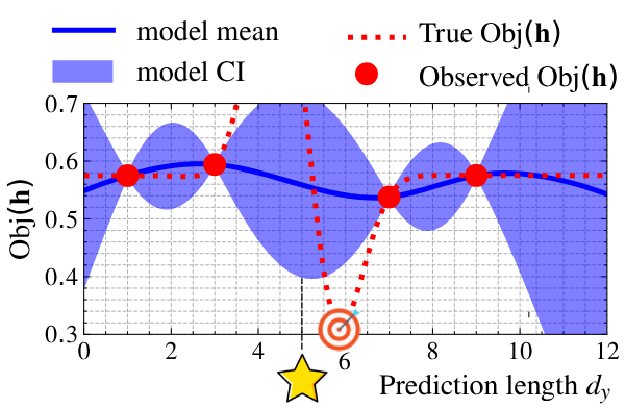
\includegraphics[width=0.42\textwidth]{img/gp_toy_example.pdf}
\caption{Bayesian optimization toy example. The star indicates the next value to try ($d_y = 5$). The target signifies the goal of minimizing the objective function.}
\label{fig:gp_toy_example}
\end{figure}

\section{PERFORMANCE EVALUATION}
\label{sec: Performance Evaluation}

This section offers a comprehensive evaluation of the proposed solution, OmniFORE, detailing the dataset used, the benchmark SoA algorithms, the experimental setup, a multitude of evaluation scenarios, and an in-depth discussion of the results obtained.

\subsection{Benchmark Schemes}

The proposed model is evaluated against several high-performance algorithms designed to handle complex temporal and spatial dependencies in multivariate time-series data:

\subsubsection*{\textbf{LSTNet: Modeling Long- and Short-Term Temporal Patterns with Deep Neural Networks \cite{LSTNet}}}
LSTNet integrates CNNs and RNNs to capture both long-term and short-term patterns. It features a recurrent-skip component for modeling long-term dependencies and an autoregressive component to manage scale insensitivity.

\subsubsection*{\textbf{AGCRN: Adaptive Graph Convolutional Recurrent Network for Traffic Forecasting \cite{AGCRN}}}
AGCRN employs GCNs with trace-specific parameter learning and data-adaptive graph generation. This model dynamically adapts to specific patterns, excelling in various time-series forecasting tasks without requiring pre-defined graphs.


\subsection{Dataset}
\label{sec:Dataset}

The Google-Trace dataset \cite{google2019cluster} offers CPU and memory usage records from eight super cells (A-H) for May 2019, sampled every 5 minutes. Each cell contains 10,000 machines running thousands of containers, capturing diverse usage patterns critical for edge-cloud modeling and forecasting.

To rigorously evaluate our model's generalization capabilities, we partition the Google traces into two distinct sets: the \textbf{regular set} and the \textbf{zero-shot set}. The zero-shot set includes entirely new, previously unseen data, ensuring that the model has no prior exposure during training. This methodology prevents data leakage from the training set into the test set, providing a more accurate assessment of the model's generalization performance. Specifically, the model is trained on the regular set and then evaluated on the zero-shot set. Consequently, the results obtained from the zero-shot set more accurately represent the model's ability to generalize to novel, unseen data.

The regular set, composed of the \textbf{cells A-F}, is used for regular training, validation, and testing. In contrast, the zero-shot set, composed of the \textbf{cells G and H}, is reserved exclusively for zero-shot testing.

We selected 100 traces for each set to balance computational feasibility with the available hardware for training the models. This choice allows us to evaluate model performance accurately without overwhelming computational resources. The time dimension $d_t$ of the dataset was then split into training ($d_\text{train} = 0.6$), validation ($d_\text{val} = 0.2$), and test sets ($d_\text{test} = 0.2$). For a visual representation of the trace selection process, refer to Fig.~\ref{fig:proposed_solution_trace_selection}.

\subsection{Experimental Settings}
This section introduces the adopted model hyperparameters, the experimental environment, and the evaluation metrics.

\subsubsection{\textbf{Hyperparameters}}
We employ the Bayesian optimization technique described in Section \ref{sec:BayesianOptimizationWithGeneralizationObjective} to fine-tune the hyperparameters for the different models. Table \ref{table:hyperparameters} presents the hyperparameter ranges and optimized values for OmniFORE, AGCRN, and LSTNet models. These ranges, based on the original authors' recommendations \cite{AGCRN, LSTNet}, strike a balance between exploration and practicality to achieve optimal generalization across diverse datasets. The Bayesian optimization process began with 20 initial training runs, followed by 30 iterations to refine the hyperparameters. The optimal hyperparameter values for the different models are listed in the result column of Table \ref{table:hyperparameters}.

\subsubsection{\textbf{Hardware and Software Environment}}
All experiments are conducted on a server equipped with 1x NVIDIA A100 SXM GPU (40 GB memory), 30 CPU cores, 200 GiB RAM, and 512 GiB SSD. The server uses an Intel Xeon processor and runs Ubuntu 20.04.2 LTS with the GNU/Linux 5.4.0-70-generic x86\_64 kernel. All methods are implemented in Python. The LSTNet and AGCRN models, provided by their authors, have been re-implemented using PyTorch 3.2.1.

\begin{table}
\centering
\caption{Hyperparameter Ranges for Bayesian Optimization Per Model}
\label{table:hyperparameters}
\footnotesize
\begin{tabular}

\textbf{}  |  \textbf{Hyperparameter}        |  \textbf{Symbol}  |  \textbf{Range}   |  \textbf{Result} 

\rotatebox{90{OmniFORE}} 
  |  Model dimension            |  $d_{embed}$    |  (64, 512)   |  194 
  |  Sequence length            |  $d_x$         |  (24, 256)   |  98  
  |  Prediction length          |  $d_y$         |  (12, 64)    |  14  
  |  Dropout rate               |  $h_{1}$       |  (0.15, 0.4)  |  0.161 
  |  Feedforward dim.           |  $h_{2}$       |  (128, 512)  |  356 
  |  Encoder layers             |  $h_{3}$       |  (1, 4)      |  2   
  |  Decoder layers             |  $h_{4}$       |  (1, 3)      |  1   
  |  Attention heads            |  $h_{5}$       |  (4, 16)     |  6   
  |  Label length               |  $h_{6}$       |  (32, 64)    |  48  
  |  Batch size                 |  $h_{7}$      |  (16, 64)    |  47  

\rotatebox{90{AGCRN}} 
  |  Embedding  dim.        |  $d_{embed}$   |  (2, 30)     |  3   
  |  Sequence length            |  $d_x$         |  (12, 72)    |  48  
  |  Prediction length          |  $d_y$         |  (12, 72)    |  22  
  |  RNN units                  |  $h_{8}$      |  (50, 200)   |  76  
  |  Number of layers           |  $h_{9}$      |  (1, 3)      |  1   
  |  Chebyshev order  |  $h_{14}$     |  (1, 3)      |  1   
  |  Batch size                 |  $h_{10}$      |  (16, 64)    |  25  

\rotatebox{90{LSTNet}} 
  |  Sequence length            |  $d_x$         |  (144, 192)  |  161 
  |  Prediction length          |  $d_y$         |  (6, 12)     |  11  
  |  Dropout rate               |  $h_{11}$      |  (0.1, 0.2)  |  0.13 
  |  CNN hidden units           |  $h_{12}$      |  (20, 143)   |  50  
  |  RNN hidden units           |  $h_{13}$      |  (20, 143)   |  107 
  |  CNN kernel size            |  $h_{14}$      |  (6, 18)     |  14  
  |  Highway window size        |  $h_{15}$      |  (24, 168)   |  93  
  |  Batch size                 |  $h_{16}$      |  (16, 64)    |  33  
  |  Skip length                |  $h_{17}$      |  (24, 24)    |  24  
  |  Skip hidden units          |  $h_{18}$      |  (20, 100)   |  77  

\end{tabular}
\end{table}


\subsubsection{\textbf{Evaluation Metrics}}
The performance of all schemes is evaluated considering the following metrics.

\paragraph*{Mean Absolute Error (MAE)}
This metric measures the average magnitude of errors without considering their direction, making it useful for assessing overall accuracy. The MAE is calculated as
\begin{equation}
  \text{MAE} = \frac{1}{n \times d_y} \sum_{i=1}^{n} \sum_{t=1}^{d_y} \left| \hat{T}_i(t) - T_i(t) \right|.
\end{equation}

\paragraph*{Root Mean Square Error (RMSE)}
This metric highlights larger errors, making it particularly effective for datasets with significant fluctuations. The RMSE is given by
\begin{equation}
  \text{RMSE} = \sqrt{\frac{1}{n \times d_y} \sum_{i=1}^{n} \sum_{t=1}^{d_y} \left( \hat{T}_i(t) - T_i(t) \right)^2}.
\end{equation}

\paragraph*{Symmetric Mean Absolute Percentage Error (SMAPE)}
This percentage-based metric is useful for comparing accuracy across different scales. The SMAPE is defined as
\begin{equation}
  \text{SMAPE} = 2 \cdot \frac{100\%}{n \times d_y} \sum_{i=1}^{n} \sum_{t=1}^{d_y} \frac{\left| \hat{T}_i(t) - T_i(t) \right|}{\left( \left| \hat{T}_i(t) \right| + \left| T_i(t) \right| \right)}.
\end{equation}

\paragraph*{Inference Time}
Inference time refers to the average duration the model requires to process its inputs and generate an output. This metric is crucial for applications demanding real-time predictions.

\paragraph*{Convergence Speed}
Convergence speed evaluates how quickly a model's training process stabilizes. A patience parameter of three is employed, ceasing training if the validation loss does not improve over three epochs. Performance is assessed using the test set RMSE after convergence to ensure robust generalization to unseen data. Lower metric values indicate better performance, providing a comprehensive evaluation of prediction accuracy and reliability.

\subsection{Experimental Results}
\label{sec: Experimental Results}

In this section, we present our evaluation results, demonstrating that the proposed model outperforms existing algorithms across all criteria. OmniFORE consistently shows lower error rates, better generalization on new data, and faster inference times. It is minimally impacted by dynamic workload changes and effectively handles trace variance, maintaining lower errors in diverse scenarios. Additionally, OmniFORE converges faster than current algorithms, highlighting its robustness and efficiency.

\subsubsection{\textbf{Hyperparameter Sensitivity and Optimization Effectiveness}}

We evaluate the sensitivity of the models to hyperparameters to gauge the effectiveness of our optimization approach from Section \ref{sec:BayesianOptimizationWithGeneralizationObjective}. Using the hyperparameter ranges $h_i$ specified in Table \ref{table:hyperparameters}, we measure performance. Figure \ref{fig:test_rmse_distribution_histogram} depicts the effect of hyperparameter tuning on test RMSE for OmniFORE, AGCRN, and LSTNet models.

OmniFORE achieves a mean test RMSE of $2.99 \times 10^{-4}$ with a standard deviation of $7.22 \times 10^{-4}$, and a factor difference (max/min) of 38.45. AGCRN records a mean test RMSE of $4.56 \times 10^{-4}$ with a standard deviation of $7.89 \times 10^{-4}$. LSTNet reports a mean test RMSE of $5.78 \times 10^{-4}$ and a standard deviation of $1.25 \times 10^{-3}$.

OmniFORE exhibits the lowest mean test RMSE and standard deviation, suggesting superior performance and reduced sensitivity to hyperparameters. However, precise tuning enhances OmniFORE's performance by a factor of 38.45, underscoring the significance of our custom Bayesian optimization for achieving robust generalization.

\begin{figure}\centering%[H]
\centering
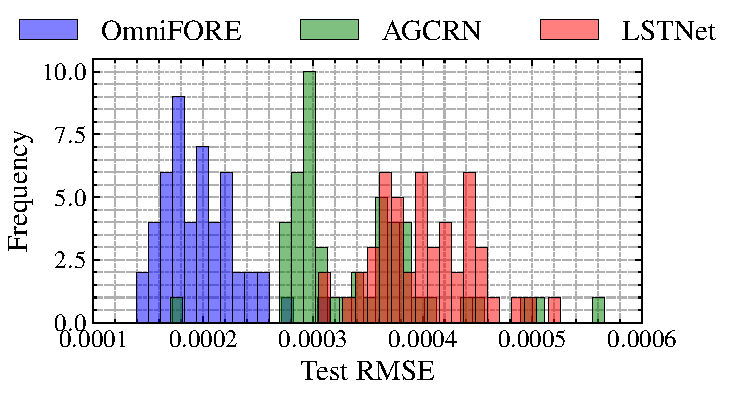
\includegraphics[width=0.49\textwidth]{img/test_rmse_distribution_histogram.pdf}
\caption{Sensitivity to Hyperparameters for Model Generalization}
\label{fig:test_rmse_distribution_histogram}
\end{figure}

\subsubsection{\textbf{Generalization Performance}}
\label{sec: Evaluation - Generalization Performance}
\paragraph*{Regular Training}
Figure \ref{fig:metrics_comparison_regular} displays the prediction performance of various models on test data from Google Cells A-F after regular training. OmniFORE demonstrates superior performance over AGCRN and LSTNet across all evaluation metrics.

OmniFORE achieves an MAE of $8.53 \times 10^{-4}$, RMSE of $5.50 \times 10^{-3}$, and SMAPE of 11.21\%. In contrast, AGCRN records an MAE of $1.04 \times 10^{-3}$, RMSE of $5.98 \times 10^{-3}$, and SMAPE of 37.19\%. LSTNet reports an MAE of $2.10 \times 10^{-3}$, RMSE of $9.21 \times 10^{-3}$, and SMAPE of 23.52\%. OmniFORE's MAE is 18.21\% lower than AGCRN and 59.42\% lower than LSTNet. Its RMSE is 7.97\% lower than AGCRN and 40.21\% lower than LSTNet. OmniFORE's SMAPE is 69.86\% lower than AGCRN and 52.34\% lower than LSTNet. This notable improvement is attributed to OmniFORE's advanced attention mechanism, which captures both long-term and short-term correlations among workloads.

Furthermore, OmniFORE achieves these results with an average inference time of \SI{8.70}{\milli\second}, compared to \SI{131}{\milli\second} for AGCRN and \SI{10.6}{\milli\second} for LSTNet. This represents a 17.92\% reduction in inference time compared to the best-performing SoA scheme, highlighting OmniFORE's efficiency for real-time applications where quick orchestration decisions are required with minimal resource overhead \cite{9500858, 8334540}. This efficiency is thanks to OmniFORE's use of generative inference, which predicts the entire sequence in a single step rather than sequentially.

\begin{figure}\centering%[H]
\centering
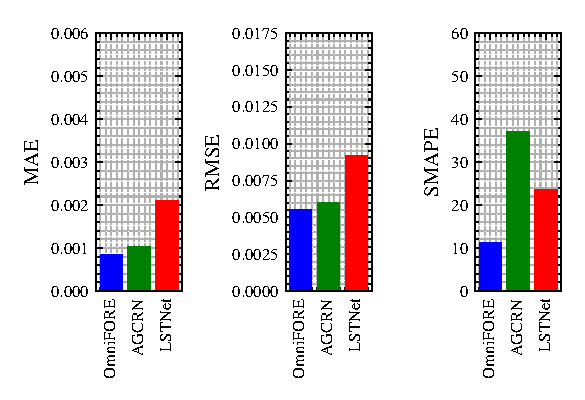
\includegraphics[width=0.49\textwidth]{img/metrics_comparison_regular.eps}
\caption{Generalization performance comparison of MAE, RMSE and SMAPE for each model for the \textbf{regular training} traces.}
\label{fig:metrics_comparison_regular}
\end{figure}

\paragraph*{Zero-Shot Performance}
Figure \ref{fig:metrics_comparison_ZS} illustrates the prediction performance using zero-shot test data from Google Cells G and H. OmniFORE achieves an MAE of $6.34 \times 10^{-4}$, RMSE of $2.92 \times 10^{-3}$, and SMAPE of 6.31\%. In comparison, AGCRN records an MAE of $3.93 \times 10^{-3}$, RMSE of $9.65 \times 10^{-3}$, and SMAPE of 55.27\%, while LSTNet shows an MAE of $5.02 \times 10^{-3}$, RMSE of $1.49 \times 10^{-2}$, and SMAPE of 39.91\%.

OmniFORE's superior zero-shot performance, surpassing even its regular training performance, stems from its advanced attention-based mechanism that captures complex patterns and dependencies, enabling robust generalization. In contrast, AGCRN and LSTNet perform worse on zero-shot data, indicating potential benefits from information leakage between training and test sets. Additionally, data variability and the exact nature of loaded traces can influence performance outcomes.

\begin{figure}\centering%[H]
\centering
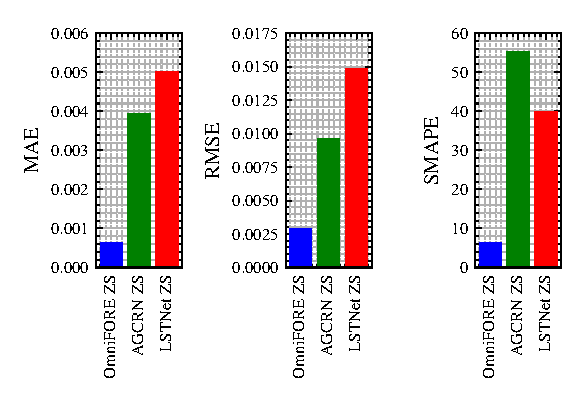
\includegraphics[width=0.42\textwidth]{img/metrics_comparison_zs.eps}
\caption{Generalization performance comparison of MAE, RMSE, and SMAPE for each model on the \textbf{zero-shot} traces.}
\label{fig:metrics_comparison_ZS}
\end{figure}


\subsubsection{\textbf{Impact of Prediction Length on Inference Time}}

In the millisecond regime, longer prediction lengths are particularly advantageous \cite{9500858}. Short-term predictions require frequent adjustments, leading to higher computational overhead and inefficiencies. In contrast, longer-term predictions enhance stability and responsiveness, allowing for smoother and more strategic resource management. This reduces the need for constant real-time recalibration and optimizes overall performance in edge-cloud environments.

As shown in Figure \ref{fig:pred_vs_inf}, we study the inference time (left subplot) and the performance in terms of RMSE (right subplot) over different prediction lengths. The inference time subplot reveals that LSTNet's computation time significantly increases with prediction length, reaching \SI{240}{\milli\second} for a length of 300, making it unsuitable for real-time applications that require latency within the \SI{50}{\milli\second} limit \cite{8334540}. In contrast, OmniFORE maintains low inference times, from \SI{12.7}{\milli\second} for a length of 5 to \SI{34}{\milli\second} for 300, thanks to efficient attention mechanisms and fast decoding. AGCRN's inference time also rises with longer predictions, reaching \SI{56}{\milli\second} for 300, which exceeds the real-time requirement, but remains higher than OmniFORE. Overall, OmniFORE is approximately twice as fast as AGCRN across all prediction lengths while maintaining performance, as evidenced by the RMSE results in the right subplot.

OmniFORE consistently outperforms AGCRN and LSTNet in RMSE, demonstrating superior accuracy. AGCRN's RMSE is generally low performant. OmniFORE's combination of low inference time and high accuracy makes it ideal for real-time, dynamic applications, outperforming both AGCRN and LSTNet.

\begin{figure}\centering%[H]
\centering
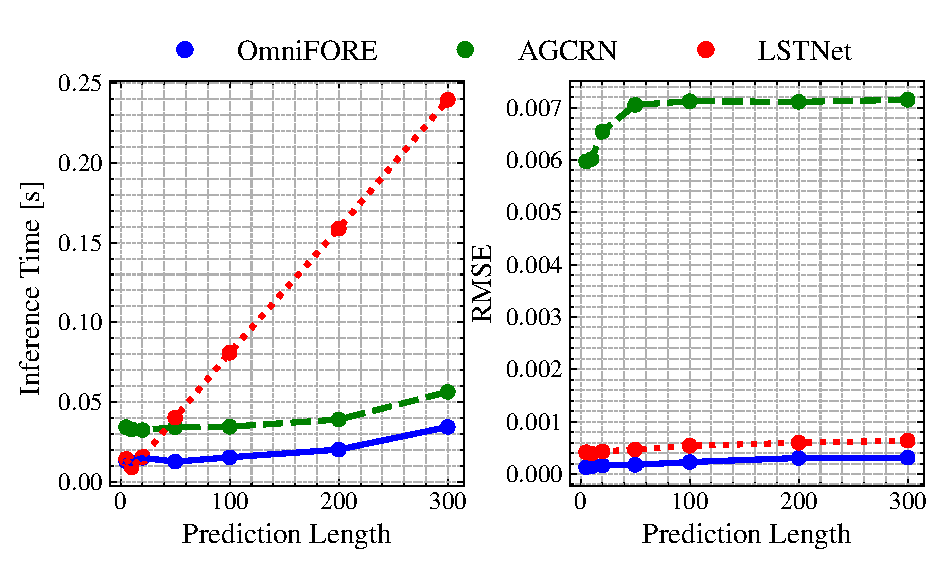
\includegraphics[width=0.42\textwidth]{img/pred_vs_inf.eps}
\caption{Impact of prediction length on inference time and RMSE for OmniFORE, AGCRN, and LSTNet.}
\label{fig:pred_vs_inf}
\end{figure}
\subsubsection{\textbf{Periodic Dynamic Workload Changes with Long-term Dependencies}}

To rigorously test OmniFORE's attention mechanism and its capacity to capture long-range dependencies, we design a signal with frequent, highly dynamic changes based on the workload diversity described in Section~\ref{sec: System Model} (Fig. \ref{fig:dynamic_workload_changes}). The signal's periodic nature, alternating between low and high usage over extended cycles, challenges the model to recognize and utilize information from distant time steps, rigorously evaluating its long-term pattern recognition capabilities.

The workload components are defined as 
\begin{equation}
T(t) = \mu \left( \sin(2\pi f t) \cdot \mathbf{1}_{\{t \% (1/f) < 0.5\}} + \mathcal{N}(0, \sigma) \right),
\end{equation}
where $\mu$ represents the mean value for the workload, $f$ is the frequency, and $\sigma$ is the standard deviation. The indicator function $\mathbf{1}_{\{t \% (1/f) < 0.5\}}$ ensures that the sine wave is active for half of its period. $\mathcal{N}(0, \sigma)$ represents Gaussian noise with a mean of 0 and standard deviation $\sigma$. The overall workload signal is generated by combining a low and high workload component:
\begin{equation}
T(t) = \begin{cases} 
T_{\text{low}}(t), & \text{if } t < \text{pattern\_length} / 2 \\
T_{\text{high}}(t), & \text{otherwise}
\end{cases}
\end{equation}
where pattern\_length = 48, representing a 2-hour cycle with 5-minute intervals.
For the low workload component, $\mu_{\text{low}} = 0.01$, $f_{\text{low}} = 0.5$, and $\sigma_{\text{low}} = 0.002$. For the high workload component, $\mu_{\text{high}} = 0.08$, $f_{\text{high}} = 1.0$, and $\sigma_{\text{high}} = 0.01$. The final workload is then adjusted to ensure positive values:

\begin{equation}
T_{\text{final}}(t) = T(t) + \mu_{\text{low}}.
\end{equation}

The connection between these equations and the input sequence lengths ($d_x$) lies in the periodic nature of the generated data. Each data point represents a 5-minute interval, making the input sequence lengths for OmniFORE (98 intervals), AGCRN (48 intervals), and LSTNet (161 intervals) (see Table \ref{table:hyperparameters}), adequate to capture the recurring patterns of the workload cycles.

Analysis of OmniFORE, AGCRN, and LSTNet reveals that OmniFORE consistently outperforms the other models. OmniFORE achieves an RMSE of 0.0322, compared to 0.0440 for AGCRN and 0.0806 for LSTNet. The lower RMSE indicates that OmniFORE's predictions have smaller average deviations from the true values, demonstrating its superior accuracy in capturing the dynamic workload patterns.

OmniFORE's advanced attention mechanism demonstrates a superior ability to understand long-term dependencies, enabling it to accurately predict dynamic changes in the workload. This capability is evident in its precise anticipation of transitions between low and high workload periods. In contrast, AGCRN and LSTNet exhibit limitations in capturing these long-range patterns, resulting in greater deviations from the true values, particularly during workload transitions. LSTNet's performance is hindered by its inability to effectively model dependencies beyond approximately 40 data points, a consequence of the vanishing gradient problem \cite{zhou2021informer}. Similarly, the CNN-based approach employed by AGCRN struggles with long-range dependencies \cite{acmtimeseriesreview2024, hochreiter1998vanishing}, impeding its ability to accurately capture and predict extended periodic patterns in the workload signal.

Notably, even in the low workload regions of the signal, OmniFORE demonstrates an understanding of the existence of minor peaks, showcasing its ability to capture fine-grained patterns in the data.

\begin{figure}\centering
\centering
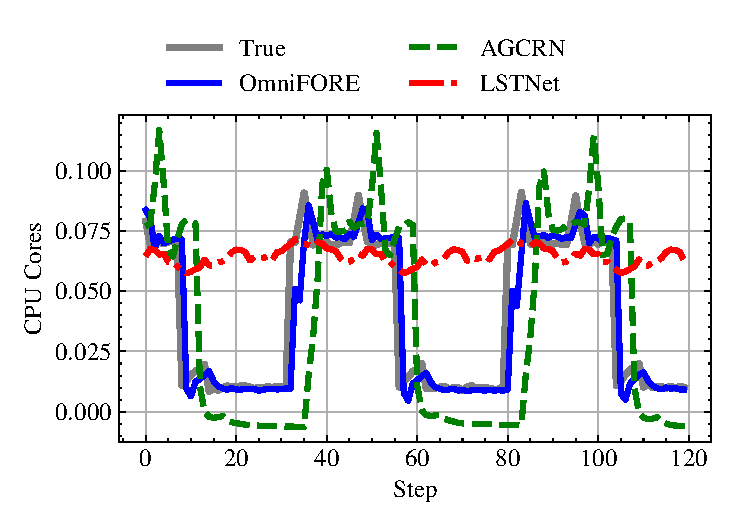
\includegraphics[width=0.42\textwidth]{img/dynamic_workload_changes.eps}
\caption{Comparison of true and predicted values for OmniFORE, AGCRN, and LSTNet under dynamic workload changes.}
\label{fig:dynamic_workload_changes}
\end{figure}

\subsubsection{\textbf{Variance-based Performance}}

We compare OmniFORE, AGCRN, and LSTNet models on both the regular CPU cores dataset and the zero-shot dataset introduced in Section \ref{sec: Evaluation - Generalization Performance} to assess their capacity to handle data with heterogeneous variance levels (Figure \ref{fig:zs_sample_trace_comparison}). OmniFORE demonstrates superior performance in capturing both low and high variance patterns, evidenced by its closer alignment with true values across diverse trace volatilities. This advantage is particularly pronounced in highly fluctuating traces, where OmniFORE maintains accuracy while AGCRN and LSTNet show increased deviations. The consistent performance of OmniFORE across both datasets underscores its robust generalization capabilities, effectively adapting to previously unseen patterns in the zero-shot scenario. 

\begin{figure}\centering%[H]
\centering
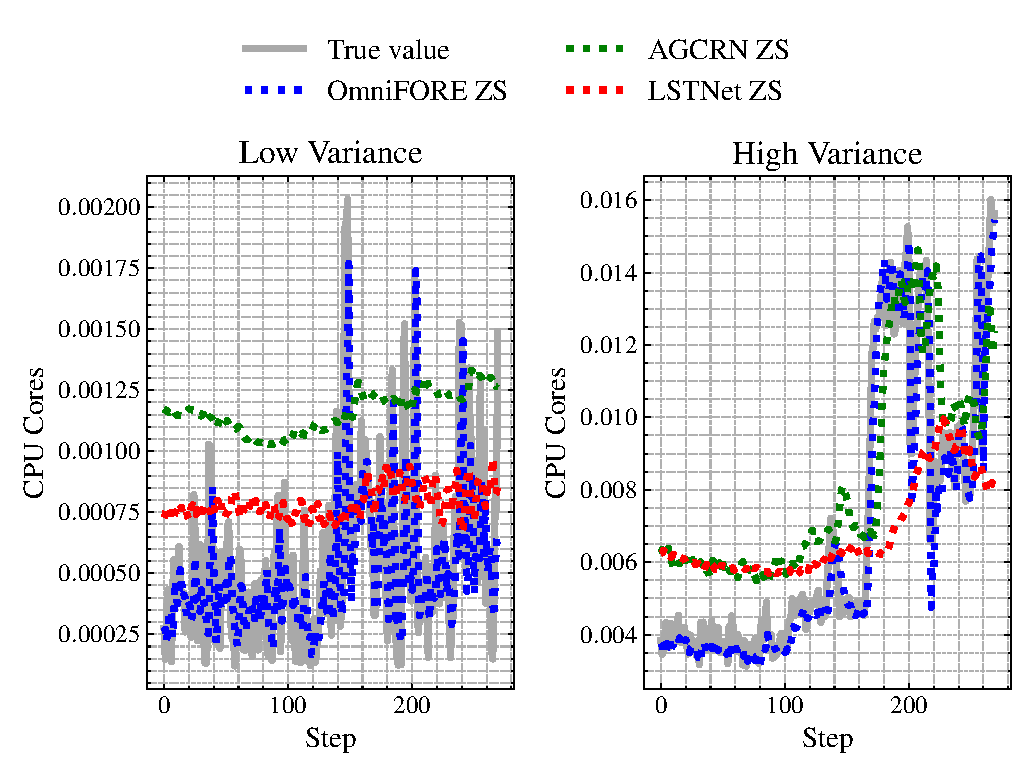
\includegraphics[width=0.42\textwidth]{img/zs_sample_trace_comparison.eps}
\caption{Comparison of true and \textbf{zero-shot} predicted values for OmniFORE, AGCRN, and LSTNet on a regular training dataset.}
\label{fig:zs_sample_trace_comparison}
\end{figure}

To further investigate, we measured the variance of each individual test trace $T_{\text{val}, i}$ and computed the performance metrics (MAE and RMSE) for these traces. Figure \ref{fig:metrics_variance_comparison_fitted} shows the relationship between trace variance and performance metrics, with linear trend lines fitted to highlight trends.

In Figure \ref{fig:metrics_variance_comparison_fitted}, slopes indicate error increase rates with rising input variance. OmniFORE exhibits the lowest slopes (regular: $1.19 \times 10^2$, zero-shot: $2.32 \times 10^1$), outperforming AGCRN (regular: $1.36 \times 10^2$, zero-shot: $2.24 \times 10^2$) and LSTNet (regular: $2.60 \times 10^2$, zero-shot: $8.75 \times 10^2$). This demonstrates OmniFORE's superior robustness to high-variance data, particularly in zero-shot scenarios.

We evaluate OmniFORE, AGCRN, and LSTNet on low and high variance traces in both regular and zero-shot scenarios. For the five lowest variance traces, OmniFORE-regular achieves an MAE of $8.96 \times 10^{-7}$, outperforming AGCRN-regular ($1.49 \times 10^{-4}$) and LSTNet-regular ($2.30 \times 10^{-6}$) by 99.4\% and 61.0\% respectively. On high variance traces, OmniFORE-regular (MAE: $1.00 \times 10^{-2}$) surpasses LSTNet-regular ($2.44 \times 10^{-2}$) by 59.0\%. In the zero-shot scenario with high variance traces, OmniFORE (MAE: $3.01 \times 10^{-3}$) outperforms AGCRN ($4.26 \times 10^{-3}$) and LSTNet ($9.05 \times 10^{-3}$) by 29.3\% and 66.7\% respectively. These results demonstrate OmniFORE's consistent superiority across diverse variance levels and generalization scenarios.

\begin{figure}\centering%[H]
\centering
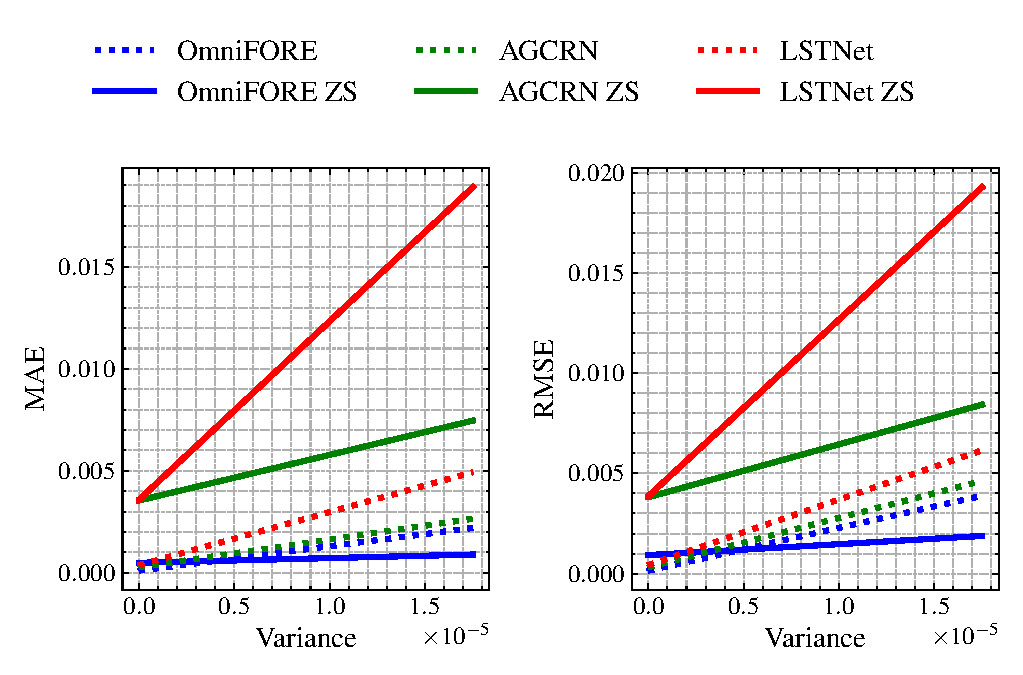
\includegraphics[width=0.47\textwidth]{img/metrics_variance_comparison_fitted2.eps}
\caption{Trace variance vs. MAE and RMSE for OmniFORE, AGCRN, and LSTNet models, with fitted linear lines.}
\label{fig:metrics_variance_comparison_fitted}
\end{figure}

\subsubsection{\textbf{Convergence}}

Quick model convergence is crucial to reduce the need for extensive training, which aids in deploying updates and maintaining overall system performance. Additionally, models that converge faster are less prone to overfitting, as they achieve their optimal state in fewer epochs.

Figure \ref{fig:test_rmse_convergence_comparison} depicts the test RMSE convergence of OmniFORE, AGCRN, and LSTNet models over multiple epochs, with early stopping applied.

OmniFORE demonstrates the fastest convergence, achieving the lowest RMSE of $5.3 \times 10^{-3}$ by the 6th epoch. LSTNet converges more gradually, reaching $8.8 \times 10^{-3}$ by the 8th epoch. AGCRN exhibits the slowest convergence, reaching $6.0 \times 10^{-3}$ by the 16th epoch.

\begin{figure}\centering%[H]
\centering
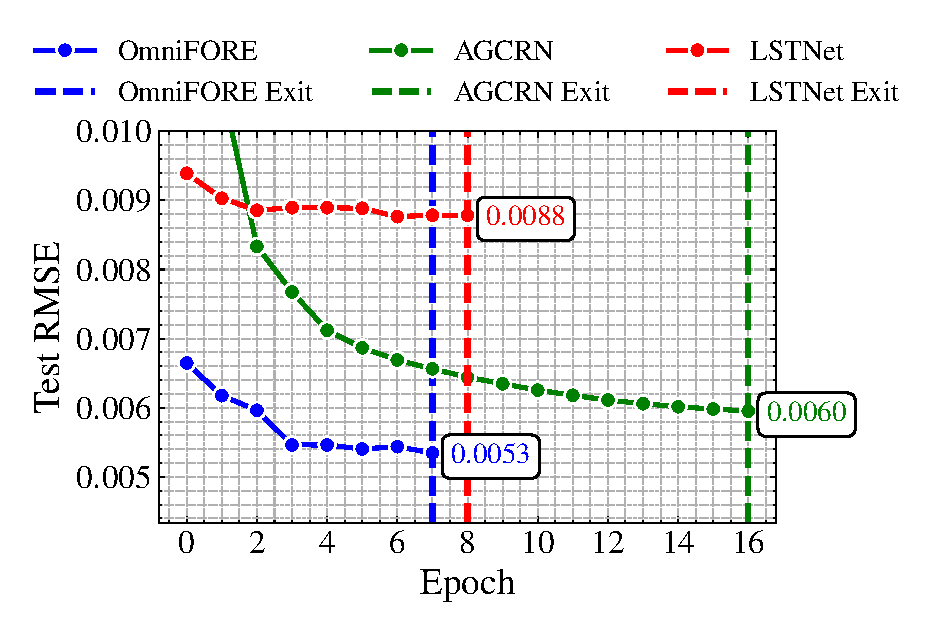
\includegraphics[width=0.49\textwidth]{img/test_rmse_convergence_comparison.eps}
\caption{Convergence of OmniFORE, AGCRN, and LSTNet models over epochs.}
\label{fig:test_rmse_convergence_comparison}
\end{figure}

% \subsection{Practical Edge-cloud Machine Learning Deployment}
% \label{sec:edge_cloud_orchestration}

% We present an advanced edge-cloud orchestration system for scalable machine learning deployment, inference, and real-time decision-making (Fig. \ref{fig:Practical_Scenario}). This architecture integrates edge computing with cloud infrastructure, optimizing both computational efficiency and resource allocation.

% \begin{figure}\centering[t]
% \centering
% 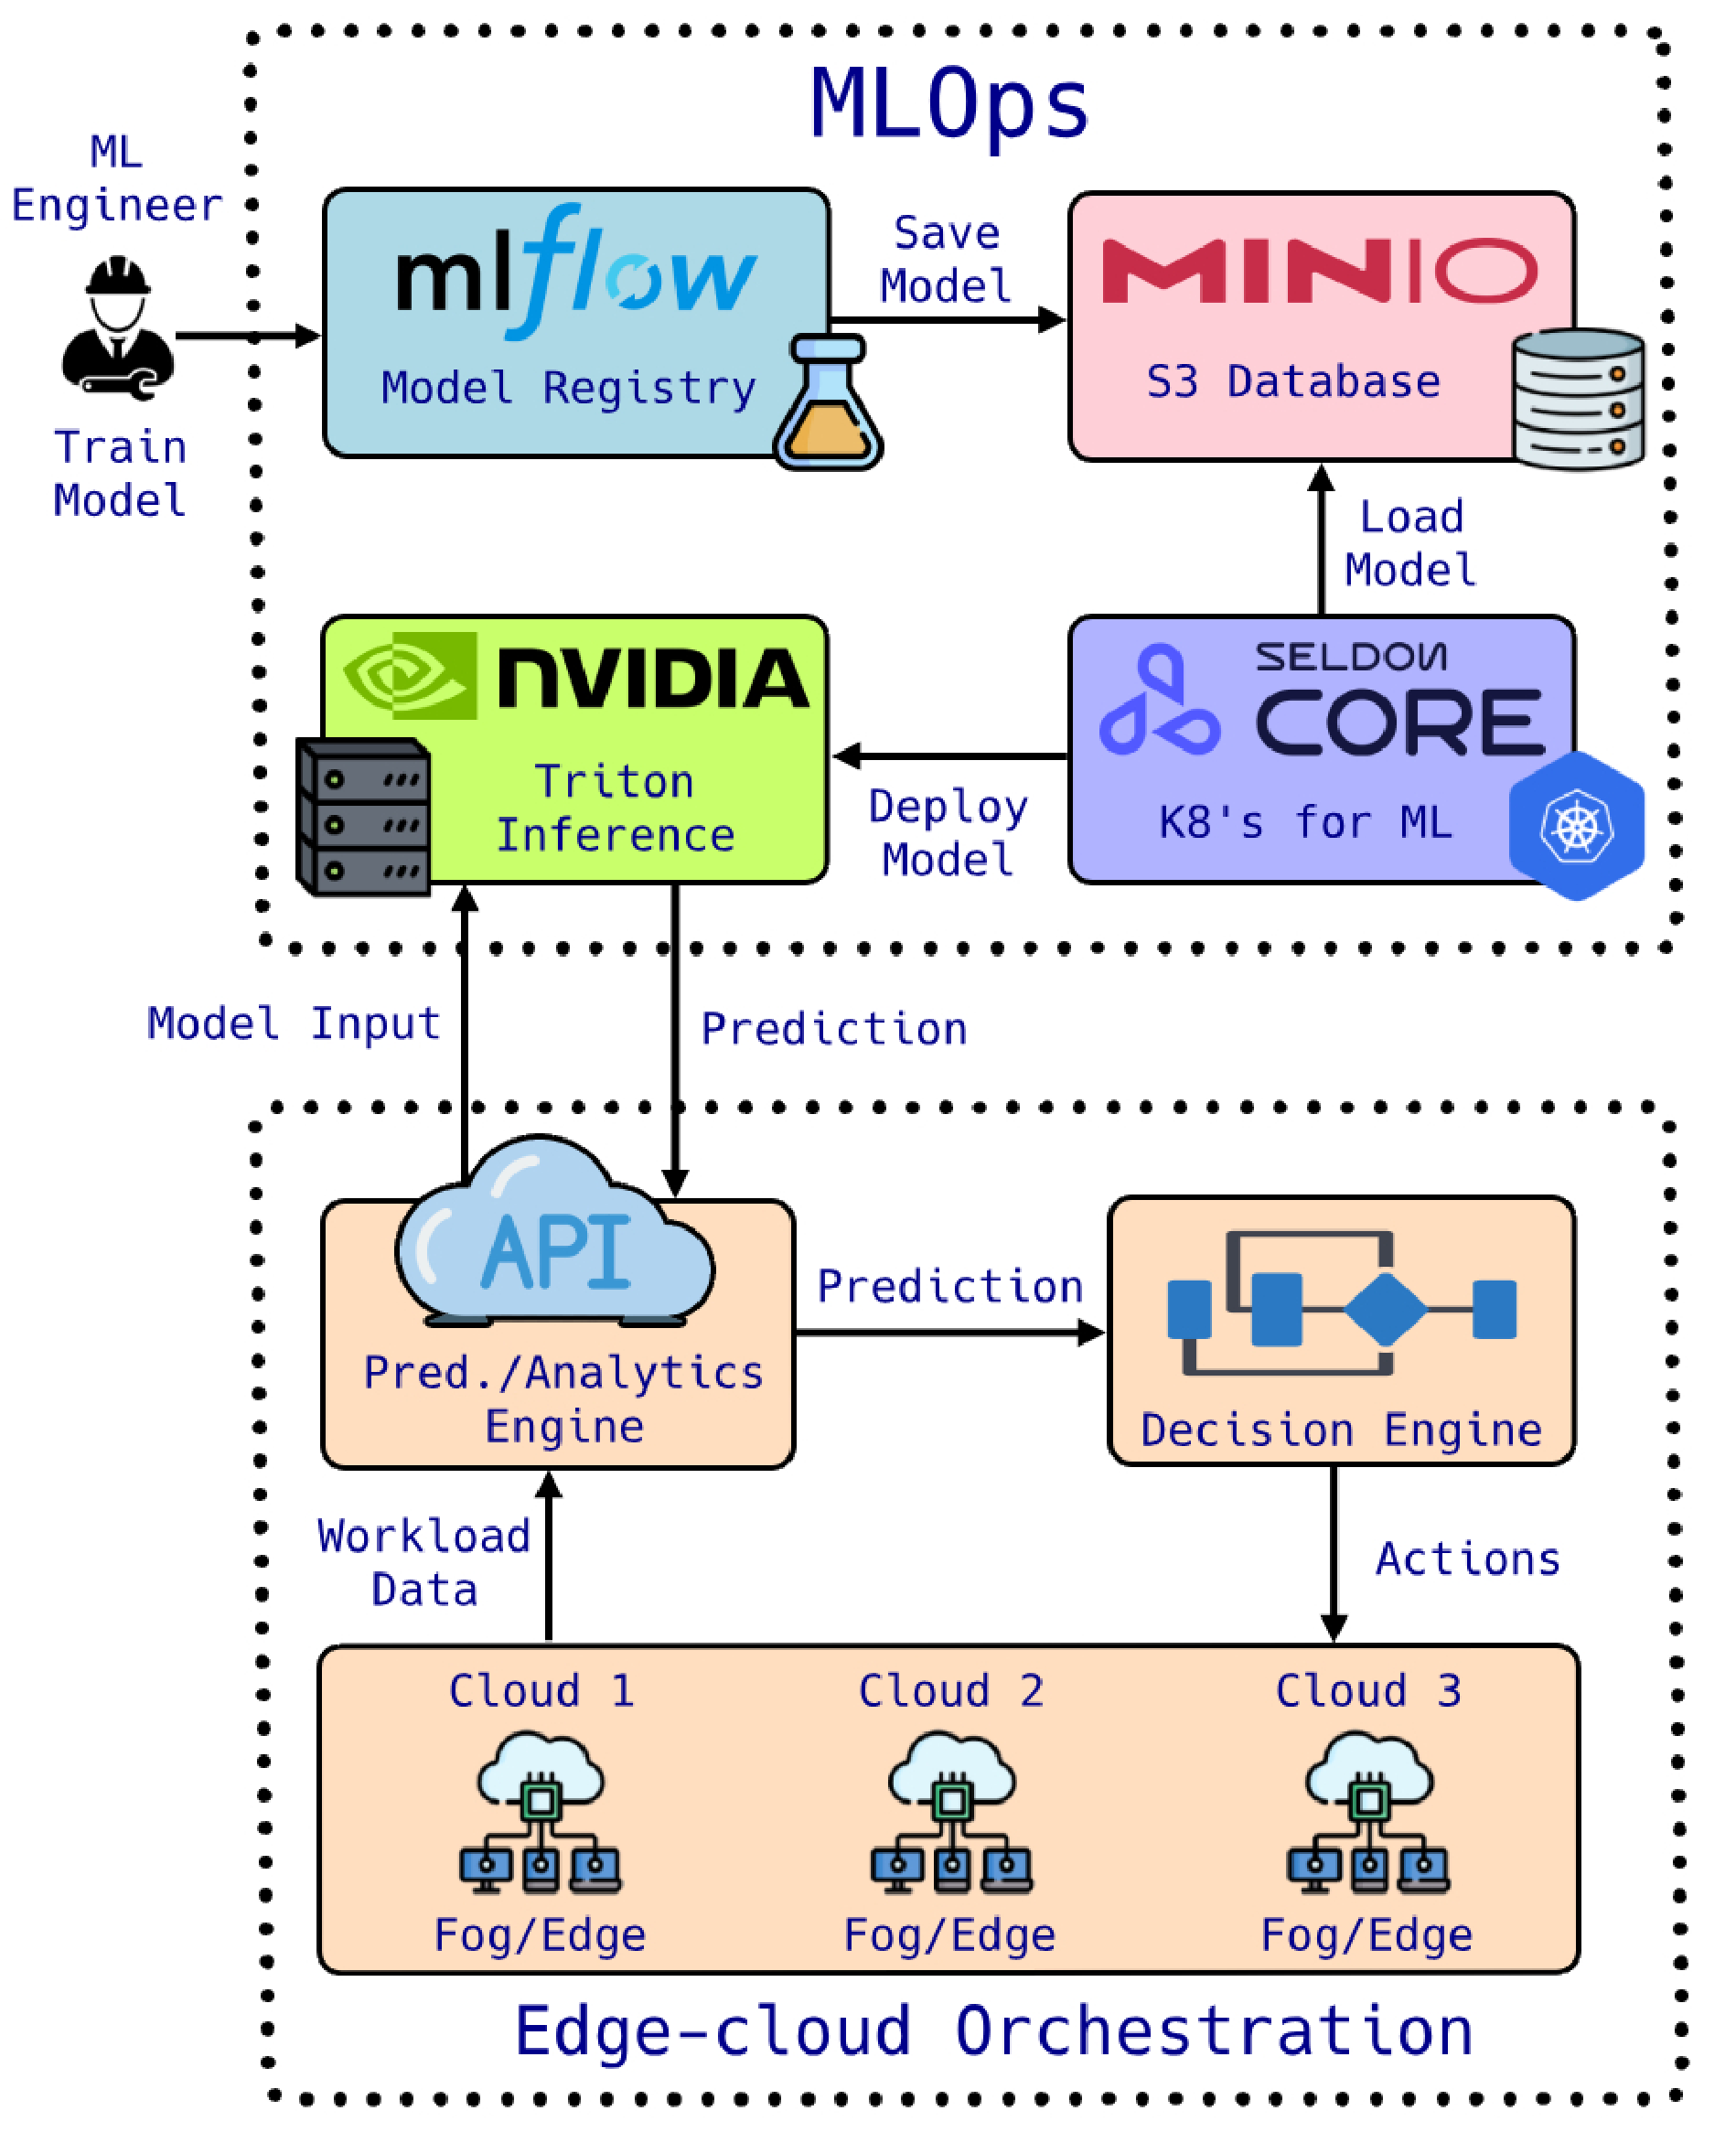
\includegraphics[width=0.47\textwidth]{img/Practical_Scenario.pdf}
% \caption{Scalable ML deployment and inference for Edge-cloud orchestration.}
% \label{fig:Practical_Scenario}
% \end{figure}

% \subsubsection{Model Development and Registry}

% Our system employs MLflow as the Model Registry, integrated with S3-compatible storage. MLflow provides robust versioning, comprehensive metadata management, and seamless integration with MLOps frameworks, facilitating reproducibility and smooth transitions from development to production across various ML frameworks.

% \subsubsection{Orchestration and Deployment}

% Kubernetes serves as the orchestration layer, managing deployment and scaling of our ML infrastructure. It offers efficient container orchestration, resource optimization, and self-healing capabilities, ensuring system reliability and scalability.

% \subsubsection{Scalable Inference}

% Scalable inference is achieved through a combination of NVIDIA Triton Inference Server and Seldon Core. Triton provides high-performance, GPU-accelerated inference with multi-framework support. It excels in concurrent model execution, dynamic batching, and supports model pipelines. Triton's HTTP/REST and gRPC inference protocols ensure broad compatibility and efficient communication.

% Seldon Core complements Triton by providing Kubernetes-native deployment for production-grade ML serving. It enables multi-model serving with efficient resource utilization, complex inference pipelines, and A/B testing capabilities. Seldon Core also offers explanation mechanisms and monitoring for deployed models.

% This combination allows for efficient deployment of diverse models from edge to cloud while maintaining high performance and scalability. A single model endpoint can serve thousands of fog/edge nodes simultaneously. This is achieved through Triton's optimized performance for various query types, combined with Seldon's ability to overcommit resources by deploying more models than available memory and unloading inactive models as needed. The result is a system capable of handling high-throughput requests from numerous edge devices efficiently.

% \subsubsection{Edge and Cloud Integration}

% Fog/Edge Nodes perform initial data processing and lightweight inference to reduce latency and minimize data transfer. Cloud Servers handle more complex computations and large-scale data analysis. A Prediction/Analytics Engine aggregates insights from both edge and cloud components, feeding into a Decision Engine for real-time decision-making.

% This architecture enables efficient, scalable, and flexible ML deployment across diverse computing environments, from resource-constrained edge devices to powerful cloud infrastructure. By leveraging Triton and Seldon Core, our system can efficiently manage thousands of fog/edge nodes from centralized model endpoints, balancing edge responsiveness with cloud computing power. The result is a robust, scalable system capable of meeting the demands of modern ML deployment scenarios across a wide range of applications and environments.

\section*{CONCLUSION}
\label{sec: Conclusion}
This paper has introduced OmniFORE, a novel framework for optimizing resource forecasts in edge-cloud networks. By combining attention-based time-series models with temporal clustering, OmniFORE achieves robust generalization and efficiently predicts diverse workloads in volatile environments. Our approach leverages strategic data sampling to extract representative traces, employs temporal clustering to differentiate workload patterns, and utilizes advanced attention mechanisms to capture both short-term and long-term dependencies. Extensive experiments on real-world datasets demonstrated that OmniFORE consistently outperforms existing benchmark schemes across various scenarios, including regular and zero-shot predictions. The framework showed significant improvements in prediction accuracy, inference speed, and adaptability to both low and high variance data. These advancements mark a substantial step forward in addressing the complexities of cloud-native workloads, paving the way for more adaptive and responsive edge-cloud systems. Future work could explore the application of OmniFORE to other domains requiring accurate time-series forecasting and investigate its potential for enhancing real-time decision-making in dynamic computing environments.

\section*{Acknowledgment}
This work is supported by the research project VERGE (SNS-JU-101096034) under Horizon Europe, and the projects AEON-ZERO (TSI-063000-2021-52), FREE-6G (TSI-063000-2021-144), AROMA3D (TSI-063000-2021-70/71), 6G-OASIS (TSI-063000-2021-24), SUCCESS-6G (TSI-063000-2021-39/40/41), AVANZANDO-5G-GEMELOS DIGITALES (TSI-063000-2021-112/113/114) under UNICO-5G-RPTR.

\bibliographystyle{format/IEEEtran}  % Choose the style, e.g., IEEE
\bibliography{references}   % Name of your .bib file

\section*{Biographies}

\begin{IEEEbiography}[{
\includegraphics[width=1in,height=1.25in,clip,keepaspectratio]{format/author1.pdf}}]
{Berend J.D. Gort}~was born in Nijmegen, Netherlands, on August 31, 1993. He received his B.Sc. and M.Sc. in mechanical engineering from TU Eindhoven, Netherlands, in 2017 and 2020, respectively, and an M.Sc. in AI \& computer engineering from Harbour.Space, Spain, in 2021. He is currently pursuing a Ph.D. in AI for 6G networking at Universitat Politècnica de Catalunya, Spain. He works as a Full-Stack Machine Learning Engineer at Nearby Computing in Barcelona, Spain, implementing time-series predictions at scale for 6G networks. His previous roles include ML Engineer at Columbia University, where he reduced overfitting in finance models by 46\%, and AI Robotics Engineer at TNO for laser-satellite communications. His research interests include machine learning for time-series forecasting. Gort is a member of IEEE, ACM, and AAAS. He has been awarded the Magna Cum Laude AI \& Computer Science honor.
\end{IEEEbiography}%


\begin{IEEEbiography}[{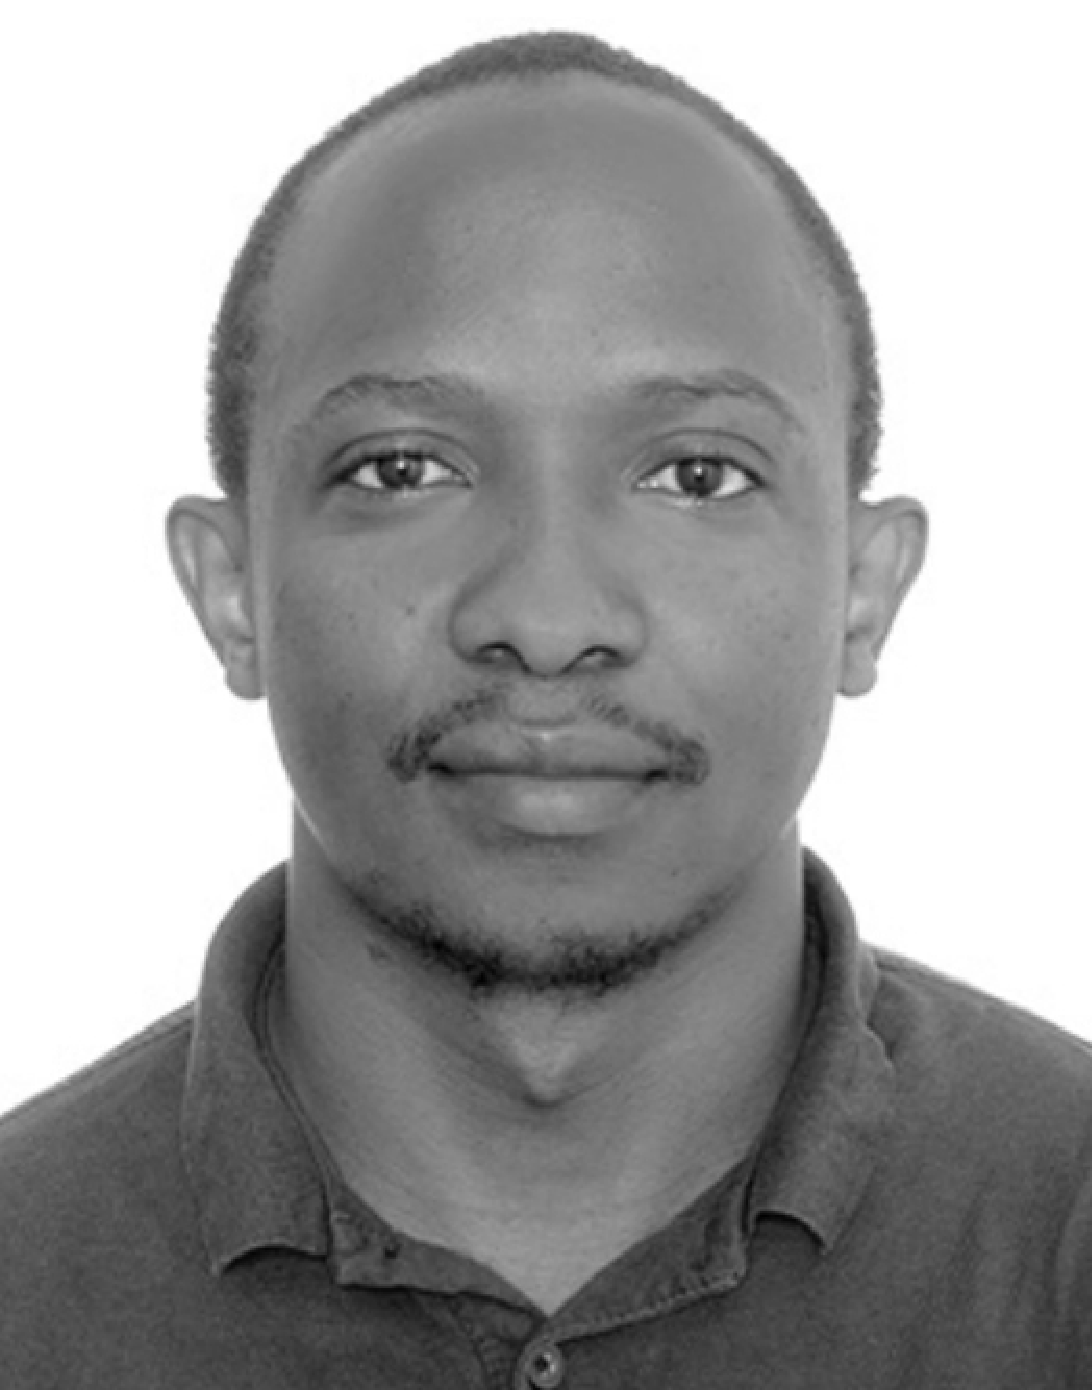
\includegraphics[width=1in,height=1.25in,clip,keepaspectratio]{format/author2.pdf}}]
{Dr. Godfrey M. Kibalya}~received his B.Sc. degree in telecommunications engineering from Makerere University, Uganda, in 2010, his M.Sc. degree in telecommunications engineering from the University of Trento, Italy, and his Ph.D. degree in network engineering from the Technical University of Catalonia (UPC), Spain. He is a Senior Researcher at Nearby Computing and an Assistant Lecturer in the Department of Electrical Engineering at Kabale University, Uganda. His previous experience includes work in telecommunications engineering in Uganda. Dr. Kibalya's research interests focus on network function virtualization and the application of artificial intelligence in network management. He is actively involved in advancing the field of telecommunications through his research and teaching roles.
\end{IEEEbiography}%

\begin{IEEEbiography}
[{
\includegraphics[width=1in,height=1.25in,clip,keepaspectratio]{format/author3.pdf}}]
{Dr. Angelos Antonopoulos}~(Senior Member, IEEE) is currently the Research and Innovation Director
at Nearby Computing S.L. He has authored over 130 papers on various topics, including multi-access edge computing, 5G/6G network architectures, network virtualization/slicing, 5G-ready vertical and over-the-top applications, zero-touch service orchestration, and analytical modeling/optimization in mobile networks.
He has received the Best Paper Award at IEEE GLOBECOM 2014, the Best Demo Award at IEEE CAMAD 2014, and the EURACON Best Paper Award at EuCNC 2016. He has been awarded with the First Prize in the IEEE ComSoc Student Competition (as a Mentor), while he was the Director of the Best UPC Thesis in ICT (2018). He has been on the editorial board of the IEEE Access, IEEE Networking Letters, Computer Networks (Elsevier), and Inventions (MDPI). He has served as officer (Secretary and Vice-Chair) of the IEEE ComSoc Technical Committee on Communication Systems Integration and Modeling (CSIM) and he is an IEEE Senior Member.
\end{IEEEbiography}

\vfill\pagebreak

\end{document}
